%%
%% This is a minimal skeleton LaTeX file for EDBT Proceedings papers.
%%
%% It uses the (somewhat) current ACM `sigconf' style with modifications
%% for EDBT Proceedings to be published on OpenProceedings.org
%%
%% You will need (apart from the ACM style) two EDBT-specific files:
%%
%% openproceedings.png   -- the OpenProceedings.org logo to be placed
%%                          on the top right corner of the first page
%%
%% edbt-macros-v29-n1.tex -- settings for Volume 29, Number 1
%%

\documentclass[sigconf]{acmart}

\usepackage{multicol}
\usepackage{multirow}
\usepackage{xcolor, colortbl}
\usepackage[linesnumbered,ruled,vlined,algoruled,boxed,noline,noend]{algorithm2e}

\usepackage{pgfplots}
\usepackage{tikz}
\usetikzlibrary{patterns}
\pgfplotsset{compat=1.15}

\usepackage{array}
\usepackage{makecell}
\usepackage{subcaption}

\usepackage{tabularx}   % For tabularx environment
\usepackage{booktabs}   % For \toprule, \midrule, \bottomrule
\usepackage{multirow}   % For \multirow
\usepackage[table]{xcolor}


%% copied from acmart.cls, but modified to a4paper
\geometry{twoside=true, head=13pt,
     a4paper, % for EDBT: use A4 paper
%     paperwidth=8.5in, paperheight=11in,
     includeheadfoot, columnsep=2pc,
     top=57pt, bottom=73pt, inner=54pt, outer=54pt,
     marginparwidth=2pc,heightrounded
     }%

\AtBeginMaketitle{%
  %% EDBT Conference Proceedings setup for ACM sigconf Style
%% Version 1.0, 2025-05-22
%% Marc H. Scholl
%%
%% \input this file within the \AtBeginMaketitle call
%% in the beginning of ACM's sample-nonacm.sty file
%%


%% EDBT: ISBN and year have to be adapted with every Number / Volume !
%%
\setcopyright{none}
\copyrightyear{\copyright\ 2025 Copyright held by the owner/author(s).
  Published on \url{OpenProceedings.org} under ISBN 978-3-98318-102-5, series ISSN 2367-2005.
  Distribution of this paper is permitted under the terms of the
  Creative Commons license CC-by-nc-nd 4.0}
\acmYear{2025}
\acmDOI{}
\acmISBN{}


%% These commands are for a PROCEEDINGS abstract or paper.
%% EDBT: This needs adaptation every year!
\acmConference[EDBT '26]{Extending Database Technology}{24-27 March 2026}{Tampere (Finland)}
%%
%%  Uncomment \acmBooktitle if the title of the proceedings is different
%%  from ``Proceedings of ...''!
%%
%%\acmBooktitle{Woodstock '18: ACM Symposium on Neural Gaze Detection,
%%  June 03--05, 2018, Woodstock, NY}


%% EDBT:
\settopmatter{printacmref=false, printccs=false, printfolios=false}


%% EDBT:
%% Macro to make image usable as hyperlink [see http://tex.stackexchange.com/questions/31819/xelatex-includegraphics-and-hyperlink]
\newsavebox{\ximagebox}
\newlength{\ximageheight}
\newsavebox{\xglyphbox}
\newlength{\xglyphheight}
\newcommand{\xbox}[1]%
  {\savebox{\ximagebox}{#1}%
  \settoheight{\ximageheight}{\usebox{\ximagebox}}%
  \savebox{\xglyphbox}{\color{white}\char32}%
  \settoheight{\xglyphheight}{\usebox{\xglyphbox}}%
  \raisebox{\ximageheight}[0pt][0pt]{\raisebox{-\xglyphheight}[0pt][0pt]{%
    \makebox[0pt][l]{\usebox{\xglyphbox}}}}%
    \usebox{\ximagebox}%
    \raisebox{0pt}[0pt][0pt]{\makebox[0pt][r]{\usebox{\xglyphbox}}}}

%% now use this to define the logo header:

\newsavebox{\LogoBox}
\sbox{\LogoBox}{
\includegraphics[height=1cm]{OpenProceedings.png}}

%% now define our header and footer for the first page
\fancypagestyle{firstpagestyle}{%
  \fancyhf{}%
  \fancyfoot{}%
  \fancyhead[L,C]{}
  \fancyhead[R]{\href{https://OpenProceedings.org/}{\raisebox{15pt}[0pt][0pt]{\xbox{\usebox{\LogoBox}}}}}
  }

\hypersetup{%
  pdfcopyright={CC-by-nc-nd}
}

}% \AtBeginMaketitle

%% end of the preamble, start of the body of the document source.

\begin{document}

%%
%% The "title" command has an optional parameter,
%% allowing the author to define a "short title" to be used in page headers.
%%
%% EDBT rule: --> Please use ``titlecase'' in the title!

\title{ALOG: Adaptive Longitudinal Grids for Geospatial Data using Local Differential Privacy}

%%
%% The "author" command and its associated commands are used to define
%% the authors and their affiliations.
%% Of note is the shared affiliation of the first two authors, and the
%% "authornote" and "authornotemark" commands
%% used to denote shared contribution to the research.
%%
%% EDBT rule: --> At least 1 (the corresponding) author needs to have a
%%                registered ORCID, ideally all authors have one
\author{Eduardo R. Duarte Neto}
\affiliation{%
  \institution{Universidade Federal do Ceará, Brazil}
  \city{Fortaleza}
  \state{Cear\'{a}}
  \country{Brazil}
}
\email{eduardo.rodrigues@lsbd.ufc.br}
\orcid{0000-0003-1222-563X}

\author{Jos\'{e} S. Costa Filho}
\orcid{0000-0002-8452-1975}
\affiliation{%
  \institution{Universidade Federal do Ceará, Brazil}
  \city{Fortaleza}
  \state{Cear\'{a}}
  \country{Brazil}
}
\email{serafim.costa@lsbd.ufc.br}

\author{Antonio A. Marreiras Neto}
\affiliation{%
  \institution{Universidade Federal do Ceará, Brazil}
  \city{Fortaleza}
  \state{Cear\'{a}}
  \country{Brazil}}
\orcid{0009-0009-0735-4964}
\email{antonio.marreiras@lsbd.ufc.br}


\author{Javam C. Machado}
\affiliation{%
  \institution{Universidade Federal do Ceará, Brazil}
  \city{Fortaleza}
  \state{Cear\'{a}}
  \country{Brazil}}
\email{javam.machado@lsbd.ufc.br}
\orcid{0000-0002-8430-9421}


%%
%% By default, the full list of authors will be used in the page
%% headers. Often, this list is too long, and will overlap
%% other information printed in the page headers. This command allows
%% the author to define a more concise list
%% of authors' names for this purpose.

\renewcommand{\shortauthors}{Duarte et al.} %%MS: removed contents
%\renewcommand{\shorttitle}{} %%MS: added this one



%%
%% The abstract is a short summary of the work to be presented in the
%% article.
\begin{abstract}
  This study introduces ALOG (Adaptive Longitudinal Grids for Geospatial Data using Local Differential Privacy), a novel framework designed to optimize geospatial data collection and frequency estimation while ensuring robust user privacy. ALOG leverages adaptive grids to dynamically adjust spatial granularity based on data density, eliminating the need for prior knowledge about data distribution. We evaluate ALOG and its variations using both synthetic and real-world datasets, comparing their effectiveness against state-of-the-art protocols. Experimental results demonstrate ALOG's superior performance in balancing privacy and utility, particularly under varying grid sizes and privacy budgets. The findings highlight the effectiveness of adaptive grid refinement in achieving precise frequency estimates in privacy-sensitive applications without relying on prior knowledge of data density. 
\end{abstract}

%% Keywords. The author(s) should pick words that accurately describe
%% the work being presented. Separate the keywords with commas.
 \keywords{Local Differential Privacy, Adaptive Grids, Geospatial Data, Frequency Estimation}

%%
%% This command processes the author and affiliation and title
%% information and builds the first part of the formatted document.
\maketitle

\section{Introduction}
\label{sec:intro}
The growing popularity of mobile devices and location-based services has led to an unprecedented influx of geospatial data, capturing detailed information on individual movements, location preferences, and popular routes \citep{Statista2015lbs,cheng2017mobile}. This surge in location data opens up opportunities for a wide range of applications across sectors, from optimizing public transportation systems and enhancing emergency response times to supporting intelligent urban planning and resource allocation \cite{ouchra2023overview}. One key approach in analyzing this data is through frequency analysis, which identifies areas with high concentrations of people over time \cite{geo_hong_21}. By quantifying how often certain locations are visited, frequency analysis provides crucial insights that enable decision-makers to allocate resources effectively and design services that meet population needs.

Frequency analysis, for instance, is widely used for generating heat maps \cite{bao2023mapping,hong2017so,peipei2020study}, which visually represent high-frequency areas or routes based on user interactions. By highlighting patterns in pedestrian traffic, vehicle concentration, or other location-based trends \cite{rikalovic2018spatial}, these maps offer actionable insights into critical areas that could benefit from additional services or infrastructural improvements \cite{miranda2023sok}. Furthermore, tracking frequency changes over time enhances understanding of dynamic trends, allowing analysis of complex, time-dependent phenomena. For instance, observing shifts in traffic flow patterns helps city planners design better road systems and optimize signal timings to alleviate congestion \cite{huang2024festgcn}. In public health, evolving frequency patterns can reveal the spread of infectious diseases \cite{bali2024exploring}, guiding officials to proactively allocate resources where they are most needed. Additionally, analyzing changes in movement patterns informs a range of personalized services and applications, from targeted advertising and location-based recommendations to social behavior research \cite{shi2020study}.

However, while these geospatial analyses offer substantial value across fields, they also raise serious privacy concerns. The data required to generate heat maps over time and track patterns often includes sensitive information about individuals' locations and movements, leading to potential risks related to user identification, behavioral profiling, and location-based discrimination \cite{unnikrishnan2013anonymizing,miranda2023sok,solymosi2023privacy}. As a result, preserving the privacy of users while leveraging the benefits of geospatial data has become a crucial issue. 

Differential Privacy (DP) has emerged as a prominent framework for enabling data analysis while preserving individual privacy \cite{DBLP:conf/icalp/Dwork06,cummings2023advancing}. However, its traditional model relies on a trusted curator, introducing potential vulnerabilities due to the risk of data breaches. To address this limitation, Local Differential Privacy (LDP) has been proposed as a robust alternative. LDP allows individuals to anonymize their data locally before sharing it for analysis, eliminating the need for a centralized curator \cite{DBLP:journals/fttcs/DworkR14,kasiviswanathan2011can}. This decentralized approach has gained significant traction in recent years, with major technology companies such as Apple \cite{DBLP:conf/uss/WangBLJ17}, Google \cite{erlingsson2014rappor}, and Microsoft \cite{DBLP:conf/nips/DingKY17} incorporating LDP into their consumer products.

LDP is particularly well-suited for scenarios involving longitudinal data—data collected from the same individual over time. For instance, in systems where users repeatedly send location reports or other personal information at multiple time intervals, the resulting data forms a longitudinal dataset. LDP ensures privacy protection in such settings by anonymizing each data point before transmission.




Despite the advantages of LDP, current techniques applied to geospatial data often rely on uniform grid structures to partition space for simplicity \cite{andres2013geo,ye2021collecting}, which can lead to an inadequate representation of the data. These approaches apply the same level of granularity to all regions, regardless of the density of points of interest, potentially compromising both the accuracy of the analyses and the utility of the aggregated data. This issue, known as non-uniformity error, arises when the assumption of uniform data distribution within grid cells does not align with the actual data distribution \cite{qardaji2013differentially}. In dense regions, this mismatch can lead to underrepresentation of critical areas, introducing bias into the results, while in sparse regions, excessive granularity can amplify noise, reducing the utility of the data. 
Because these methods don't consider how data is distributed within a region, they can produce large errors.
For example, in dense regions, uniform grids may be too coarse, leading to significant bias when answering queries. On the other hand, regions with sparse data may be mapped by a fine-grained grid, resulting in weak utility and high noise during query answering \cite{qardaji2013differentially}. \looseness=-1

In this paper, we propose a new approach based on adaptive, non-uniform grids that dynamically adjust to data point densities, allowing for greater accuracy in regions with high individual concentration and coarser granularity in less dense areas. Our methodology combines the flexibility of adaptive grids with the privacy guarantees offered by Local Differential Privacy. By iteratively refining cell sizes as new data is reported, our approach incrementally adjusts to temporal variations in data distribution. This temporal refinement is essential to accurately capture the correlations present among consecutive reports submitted under Local Differential Privacy (LDP), enabling our framework to deliver more precise and context-aware analyses. Thus, these enhancements make our framework, called ALOG (Adaptive Longitudinal Grids), particularly well-suited for addressing the challenges of privacy-preserving geospatial data analysis.
% 
\subsubsection*{Contributions} In summary, this paper makes the following contributions:\looseness=-1
\begin{itemize}
    \item We propose ALOG, an adaptive grid-based framework for LDP-compliant longitudinal data collection, which exploits temporal correlations and dynamically refines spatial partitions to balance privacy and utility. 
    \item  We analyze various grid refinement strategies to detect and adapt to changing patterns in data density throughout the grid adaptation windows with a detailed investigation of the factors that influence the utility-privacy trade-off.
    \item To assess the effectiveness of our adaptive longitudinal data collection framework, we conduct comprehensive evaluations using both synthetic and real-world datasets while comparing them with different prior state-of-the-art techniques.\looseness=-1
\end{itemize}

\subsubsection*{Organization} Section 2 formalizes the problem tackled in this work, and presents the foundations and essential definitions used throughout the work. In Section 3, we present
the related work and discuss how the main existing approaches
work and their limitations. We present our approach in Section 4. Experimental results are shown in Section 5. Finally, Section 6 concludes
this work.

\section{Foundations and Key Concepts}
\label{sec:background}

This work addresses the challenge of estimating the frequency of user visits within a spatial region of interest, $S$ (e.g., a city), while ensuring user privacy. The region $S$ is partitioned into a uniform grid $G$, where each cell $g_{i} \in G$ represents a distinct sub-region. For a set of users $U=\{u_{1}, u_{2}, ..., u_{n}\}$ moving within $S$ across discrete timestamps, the objective is to estimate the frequency $\hat{f}_{i}$ of visits to each cell $g_{i}$. Users generate true location reports $r_{i}$ at each timestamp, which are then anonymized locally using a Local Differential Privacy (LDP) mechanism $\Psi$ to produce private reports $\hat{r}_{i}=\Psi(r_{i})$ \cite{Filho2023FELIP}. An aggregator collects these private reports $\{\hat{r}_{i}\}_{i=1}^{|U|}$ and estimates the cell frequencies $\hat{f}_{i}$ using an estimator function $F(\cdot)$. Key concepts like LDP and Frequency Estimators, detailed below, form the basis of this approach. Table~\ref{tab:notations} summarizes commonly used notations. 

\begin{table}[tb]
  % \footnotesize
  \caption{Commonly Used Notations}
  \begin{tabular}{cp{5.9cm}}
    \toprule
    Notations&Meaning\\
    \midrule
    $S$ & Geo-space \\
    $g_i$,$G_i$ & Grid cell and Grid partition of $S$\\
    $u$,$U$ & User and the set of all users \\
    $t$,$T$ & Timestamp and set of all timestamps \\
    $f_i$,$\hat{f_i}$ & Frequency and frequency estimation for cell $g_i$\\
    $r_i$,$\hat{r}_i$ & User true report and user private report at each timestamp $i$ \looseness=-1\\
    $w$, $k$ & Window and grid size\\
  \bottomrule
\end{tabular}
\label{tab:notations}
\end{table}

\subsection{Local Differential Privacy}


Local Differential Privacy (LDP) differs significantly from the centralized model of Differential Privacy (DP) \cite{DBLP:conf/icalp/Dwork06} in where data perturbation occurs. In LDP, each user applies a randomized algorithm $\Psi$ locally to perturb their true data \textit{before} it is transmitted. Only the perturbed output is sent to the server, protecting the raw data and making LDP suitable for settings without a fully trusted data curator. This model is well-suited for longitudinal data, where users repeatedly report information over time, ensuring privacy at each step \cite{arcolezi2022improving}. \looseness=-1

\begin{definition}($\epsilon$ - LDP \cite{erlingsson2014rappor}) An algorithm
$\Psi(\cdot)$ satisfies $\epsilon$-local differential privacy, where $\epsilon \geq 0$, if and
only if for any pair of inputs $(v,v')$, and any set $R$ of possible outputs
of $\Psi$, we have
\begin{equation}
Pr[\Psi(v) \in R] \leq e^\epsilon Pr[\Psi(v') \in R]
\end{equation}
\label{def_ldp}
\end{definition} 

% \vspace{-0.6cm}

Intuitively, $\epsilon$\textit{-LDP} ensures that given the perturbed output in $R$,
it is not possible for the server or for an adversary to
distinguish whether the original true value was $v$ or $v'$ beyond
the probability ratio $e^\epsilon$. Here, $\epsilon$ controls the privacy level. Lower $\epsilon$ yields
stronger privacy. Analogous to central DP, LDP also benefits from key foundational properties, including robustness to post-processing and composition \cite{DBLP:journals/fttcs/DworkR14}.\looseness=-1

\begin{proposition}(Post-Processing)
    If $\Psi$ is $\epsilon$-LDP, then $f(\Psi)$ is also $\epsilon$-LDP for any function $f$.
\label{prop:post_processing}
\end{proposition}

\begin{proposition}(Sequential Composition)
     Let each $\Psi_i$ be an $\epsilon$-LDP mechanism, and $\Psi$ is the sequential composition $\Psi_1$,...,$\Psi_m$. Then, $\Psi$ satisfies $\sum_{i=1}^{m}  \epsilon$-LDP.
\label{prop:seq_processing}
\end{proposition}

\subsection{Frequency Estimator}
\label{sec:freq_estimator}

A frequency estimator is an LDP mechanism designed to estimate how often each value $r \in V$ appears in the dataset, where $V$ is the set of all possible values of a given attribute \cite{cormode2021frequency,bassily2015local}. A frequency estimator consists of two components: A sanitizer and an aggregator. The sanitizer is employed by users to locally perturb their data. An aggregator receives the perturbed data and estimates the frequencies regarding the input. Frequency estimators have been employed for a variety of different tasks such as answering range queries \citep{Filho2023FELIP}, identifying heavy hitters \citep{heavy_hitter_Zhu_24,qin2016heavy}, and the problem we attack in this paper, namely private queries on geospatial data \citep{geo_hong_21,laouir2024diapprox,tire2024answering}. \looseness=-1
\begin{figure}[htb]
    \centering
    \Description{Frequency estimation framework}
    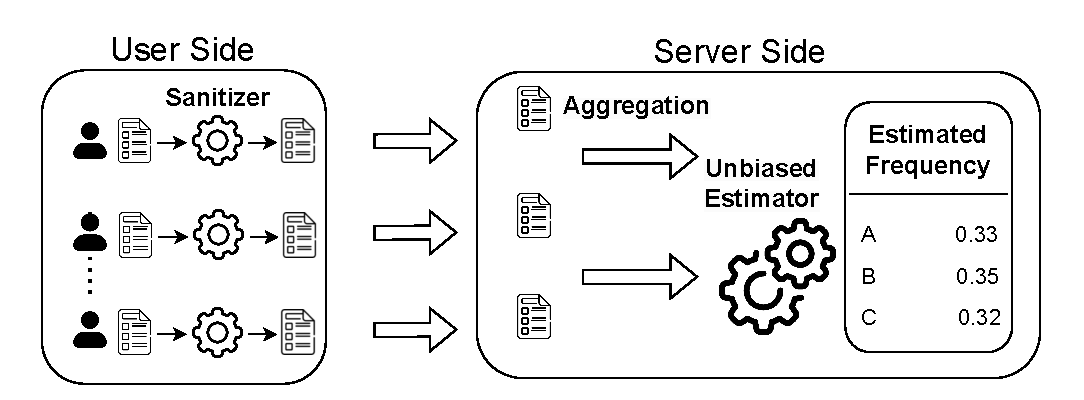
\includegraphics[width=0.9\linewidth]{sections/figures/freq_estimator.pdf}
    \caption{Frequency Estimator: users sending their sanitized report to the aggregator to estimate the frequency of values for a given attribute.}
    \label{fig:FE}
\end{figure}
% 
Figure \ref{fig:FE} illustrates a typical frequency estimator. In this example, the domain consists of three possible values: A, B, and C, which could represent items a user purchased, such as a doll, a car, or a dog. Each user applies a sanitization mechanism to their true report before submitting the sanitized version to the server. On the server side, the aggregator collects all sanitized reports and estimates the frequency of each value in the domain.

\subsection{Space Partitioning}
\label{sec:space_partition}

Spatial regions are commonly represented using map projections such as the Mercator projection, which converts latitude and longitude into a planar format \cite{peterson2014mapping}. While suitable for visualization, many analytical tasks require discretizing this continuous space into manageable units. Grid-based partitioning is a widely used approach due to its simplicity and effectiveness in dividing the region into uniform, contiguous cells \cite{shekhar2011identifying}.

Each cell represents a discrete sub-region of the original space, allowing any point (latitude and longitude) to be mapped to a specific cell. This structure supports efficient spatial queries, aggregations, and systematic data processing, particularly in high-density datasets \cite{yu2018geosparkviz}. \looseness=-1

To represent positions within the grid computationally, unary encoding can be applied. In a grid with \( k \) cells, each location is represented as a binary vector of length \( k \), with a 1 indicating the active cell and 0s elsewhere. For example, if a user is in cell 20 of a 100-cell grid, their position is encoded as a 100-bit vector with a 1 at index 20. Unary encoding is well-suited for privacy-preserving applications, as it enables straightforward integration with differential privacy mechanisms \cite{yang2023local}.

By discretizing spatial data and encoding positions in this manner, it becomes possible to anonymize and aggregate location information effectively, enabling privacy-aware frequency estimation and spatial analysis in sensitive domains.




\section{Related Work}
\label{sec:related_work}

Centralized models for estimating individual frequencies in geospatial areas typically use grids to partition space for location discretization \cite{DBLP:conf/icde/QardajiYL13,wei2019differential,yan2022achieving}. Qardaji et al.  \cite{DBLP:conf/icde/QardajiYL13} address the problem of constructing a differentially private synopsis for two-dimensional datasets, such as geospatial datasets. They highlight that a key challenge is balancing noise error and non-uniformity error in partition-based synopsis methods and study the uniform-grid approach. The authors propose a method for choosing the grid size. They also introduce an adaptive-grid method that refines cell granularity based on data density. Kim et al. \cite{kim2024improving} proposes a method that combines Geo-Indistinguishability \cite{andres2013geo} with adaptive grids, adjusting grid granularity based on real-time user density to improve location-based analysis accuracy. Unlike centralized approaches, several studies have explored Local Differential Privacy (LDP) to enhance location privacy. Erlingsson et al.  \cite{erlingsson2014rappor} introduced RAPPOR, a protocol that uses LDP in longitudinal data collection. Arcolezi et al.  \cite{arcolezi2022improving} proposed L-OSUE, an enhanced LDP protocol that improves frequency estimate accuracy across time and multiple dimensions. Additionally, Arcolezi et al.  \cite{arcolezi2022frequency} developed LOLOHA, an extension of OLH, for handling evolving data in trajectory-based applications, which refines hash functions dynamically to enhance location-based analysis accuracy. Cunningham et al. \cite{cunningham2021real} propose an LDP mechanism based on perturbing hierarchically structured, overlapping n-grams of trajectory data. It uses a multi-dimensional hierarchy over real-world places of interest to improve the realism and utility of perturbed, shared trajectories.

While effective, applying LDP protocols to location privacy presents challenges. Specifically, discretizing continuous location data into a grid structure requires dynamic grid evolution to adapt to variations in user density, balancing privacy and data utility.

This work explores the use of adaptive grids with LDP protocols to improve privacy and maintain high data utility. It will be compared experimentally against state-of-the-art LDP methods, such as RAPPOR, LOSUE, and LOLOHA, to demonstrate the effectiveness of adaptive grid structures in handling evolving location-based datasets. \looseness=-1


\subsection{RAPPOR} \label{sec:rappor}
RAPPOR \citep{erlingsson2014rappor} is an influential work in the development of LDP and frequency estimators. It makes use of two rounds of sanitization and \textit{memoization} to provide LDP guarantees for several queries over time. RAPPOR is especially relevant for longitudinal location data, as it allows for ongoing collection while protecting individual privacy by encoding and perturbing the data. In the context of location data, the domain size $k$ refers to the number of possible location encodings within the grid. Each user's location at a given timestamp is encoded into this k-dimensional space, and RAPPOR's perturbation mechanisms are applied to this encoding. This process is repeated at each timestamp, allowing for frequency estimation of location visits over time while preserving privacy. 

The first round of sanitization is referred to as the PRR step (permanent randomized response), and the second as the IRR step (instantaneous randomized response), both referencing the randomized response algorithm and their respective functions. In the \textit{memoization} process, PRR adds noise to a value the first time it is processed, and then the sanitizer memoizes the noisy value, while IRR adds noise to every instance of a memoized value before sending a report to the aggregator. By memorizing a randomized version of a true value and consistently reusing it, or reusing it as input to a second round of sanitization, it becomes harder for an adversary to track changes in the data and reduces the impact of temporal correlations, making it more difficult to track changes in the data and infer the true values. As the domain size gets larger, it becomes a challenge to apply noise in a utility-preserving way, thus RAPPOR implements Unary Encoding as a means of guaranteeing LDP while reducing data utility loss. In Unary Encoding, an input value $v$ from a domain $D$ of size $k$ is encoded as a binary vector $B$ of length $k: B = [0, ..., 0, 1, 0, ..., 0]$, where only the v-th position is 1.

The perturbation protocol for RAPPOR and other UE-based LDP protocols is as follows: Given the probabilities \textit{$p_1$, $p_2$, $q_1$, $q_2$} to flip the $i$-th position of the binary vector $B$, for the first sanitization round, we have 
% 
% \begin{align*}
% Pr\bigr[\Psi_{UE_{(\epsilon)}}B'[i]=1] =
% \begin{cases}
%       p1, \text{if } B[i] = 1 \text{ and round = }1\\
%       q1, \text{if } B[i] = 0 \text{ and round = }1\\
%       p2, \text{if } B[i] = 1 \text{ and round = }2\\
%       q2, \text{if } B[i] = 0 \text{ and round = }2\\
% \end{cases},
% \end{align*}
%

\begin{align*}
Pr\bigr[\Psi_{UE_{(\epsilon)}}B'[i]=1] =
\begin{cases}
      p_1, \text{if } B[i] = 1 \\
      q_1, \text{if } B[i] = 0 \\
\end{cases},
\end{align*}


and for the second


\begin{align*}
Pr\bigr[\Psi_{UE_{(\epsilon)}}B'[i]=1] =
\begin{cases}
      p_2, if B[i] = 1\\
      q_2, if B[i] = 0\\
\end{cases},
\end{align*}
% 
\textit{$p_1$, $p_2$, $q_1$, $q_2$}  are computed as function of $\epsilon_{\infty}$ and $\epsilon_{1}$ by symmetric unary encoding (SUE) to satisfy: $p_1 = \frac{e^{\epsilon_{\infty}/2}}{e^{\epsilon_{\infty}/2} + 1}$, $q_1 = \frac{1}{e^{\epsilon_{\infty}/2} + 1}$, $p_2 = 0.75$, and $q_2=1-p_2$. 

% So $\epsilon_1 = ln\left(\frac{(p_1p_2-q_2(p_1-1))(p_2q_1-q_2(q_1-1)-1)} {(p_2q_1-q_2(q_1-1))(p_1p_2-q_2(p_1-1)-1)}\right)$.
% 
% \begin{equation}
% \small
% \label{eq:eps1_ue}
% \epsilon_1 = ln\left(\frac{(p_1p_2-q_2(p_1-1))(p_2q_1-q_2(q_1-1)-1)} {(p_2q_1-q_2(q_1-1))(p_1p_2-q_2(p_1-1)-1)}\right)
% \end{equation}
% 
$\epsilon_{\infty}$ is an upper bound for the privacy budget as the number of reports sampled by the frequency estimator tends to infinity, and $\epsilon_{1}$ is a lower bound for a single report. The value of $\epsilon_{1}$ is computed using the following equation:

\begin{equation}
% \small
\label{eq:eps1_ue}
\epsilon_1 = ln\left(\frac{(p_1p_2-q_2(p_1-1))(p_2q_1-q_2(q_1-1)-1)} {(p_2q_1-q_2(q_1-1))(p_1p_2-q_2(p_1-1)-1)}\right)
\end{equation}

All frequency estimators presented in this paper, including those based on the RAPPOR protocol discussed in this section and the L-OSUE and LOLOHA protocols covered in the following two sections, utilize the same unbiased function to estimate frequencies at the aggregator \citep{erlingsson2014rappor,arcolezi2022improving,arcolezi2022frequency}:  \looseness=-1
% 
\begin{equation}
% \small
\label{eq:round2_est}
\Phi_{f_L}(v) := \frac{C(v) - nq_1(p_2-q_2) - nq_2}{n(p_1 - q_1)(p_2 - q_2)} = \frac{{\frac{C(v)/n - q_2}{p_2 - q_2}} - q_1}{p_1 - q_1},
\end{equation}
% 
where \textit{n} is the number of reports, \textit{p1, p2} \textit{, q1, q2} are the probabilities for perturbing the data, and \textit{C(v)} is the count of reports with a value \textit{v}, given $v \in D$. \looseness=-1

\subsection{L-OSUE}
\label{sec:losue}

L-OSUE is an alternative to RAPPOR proposed in \cite{arcolezi2022improving}. It uses the OUE \cite{8253434} protocol for its first round of sanitization (PRR step) and SUE \cite{de2020protecting}, which is equivalent to simple single-time RAPPOR, for the second (IRR step). The perturbation algorithm follows the same structure as RAPPOR, but with $p_1 =0.5$, $q_1 = \frac{1}{e^\epsilon_{\infty} + 1}$, $p2=\frac{e^\epsilon\infty e^\epsilon_1-1}{e^{\epsilon_\infty} - e^\epsilon_1+e^{\epsilon_\infty +\epsilon_1}-1}$, $q_2=1-p2$, and $\epsilon_1$ calculated using equation \ref{eq:eps1_ue}. It provides better privacy guarantees than RAPPOR, while not introducing too much extra noise and preserving similar data utility. Similar to RAPPOR, L-OSUE can be applied to longitudinal location data by encoding locations into a $k$-dimensional space, where $k$ is the number of cells in the grid.  At each time step, user locations are encoded, perturbed using L-OSUE's two-round approach, and reported. This allows for improved accuracy in frequency estimates across both time and multiple dimensions, crucial for longitudinal location-based analysis.

\subsection{LOLOHA}
\label{sec:loloha}

Unlike RAPPOR and L-OSUE, LOLOHA \citep{arcolezi2022frequency} does not make use of unary encoding; it instead improves utility by shrinking the domain size through local hashing. Like the previously cited estimators, LOLOHA implements two rounds of sanitization and memoization to provide LDP guarantees while maintaining utility for queries executed over time.  In the context of location data, LOLOHA uses a hash function to reduce the domain size from $k$ (the number of grid cells) to a smaller space before applying perturbation. This hashing is crucial for managing the evolving nature of location data over time. At each timestamp, user locations are hashed, perturbed, and reported, allowing the aggregator to estimate frequency distributions accurately as new reports are continuously collected. In this paper, we will use OLOLOHA, the optimal configuration of LOLOHA. It shrinks a domain size $k$ to an optimal hashed size $g$, that is computed by 
% 
\begin{equation}
% \small
g = 1 + \max\left(1, \left\lceil \frac{1 - a^2 + \sqrt{A}}{6(a - b)} \right\rceil \right),
\label{eq:ololoha_g}
\end{equation}
where $A = a^4 - 14a^2 + 12ab(1 - ab) + 12a^3b + 1$ given $a = \epsilon_{\infty}$ and $b = e^{\alpha\epsilon_{\infty}}$ for $\alpha \in (0, 1)$.

In local hashing, given an original domain size $k$ and input values $v \in V,$ a randomly chosen universal hash function $H$ maps the original domain to a range $[1...g]$ with $g \geq 2$. Approximately $k/g$ values $v \in V $can be mapped to the same hashed value $H(v) \in [1...g]$ due to collision. The sanitization protocol for LOLOHA is as follows:
% 
\begin{align*}
\forall_{x \in [1...g]}\text{ }Pr\bigr[\Psi_{LOLOHA_{(\epsilon_\infty)}}(v) = x\bigr] =
\begin{cases}
      p_1 = \frac{e^\epsilon}{e^\epsilon + g - 1}  & \text{if x = v} \\
      q_2 = \frac{1}{e^\epsilon + g - 1} & \text{if x $\neq$ v} \\
\end{cases} 
\end{align*}
followed by a second round that outputs a report $x'$:
\begin{align*}
\forall_{x' \in [1...g]}\text{ }Pr\bigr[\Psi_{L-GRR_{(\epsilon_1)}}(x) = x'\bigr] =
\begin{cases}
      p_2 & \text{if x' = x} \\
      q_2 = \frac{1 - p_2}{g - 1} & \text{if x' $\neq$ x} \\
\end{cases} 
\end{align*}
% where $p_2 = \frac{q_1 - e^{\epsilon_1}p_1}{(-p_1e^{\epsilon_1}) + gq_1e^{\epsilon_1} - q_1e^{\epsilon_1} - p_1(g-1)+q_1}$ as $\epsilon_1 = ln(\frac{p_1p_2+q_1q_2}{p_1q_2+q_1p_2})$ for LOLOHA. \looseness=-1
where:
\begin{align*}
\epsilon_1 &= \ln\left(\frac{p_1p_2 + q_1q_2}{p_1q_2 + q_1p_2}\right), \text{ and} \\
p_2 &= \frac{q_1 - e^{\epsilon_1}p_1}{
  -p_1e^{\epsilon_1} + gq_1e^{\epsilon_1} - q_1e^{\epsilon_1} - p_1(g - 1) + q_1}.
\end{align*}

After the sanitization step, the reports, privacy budgets, and hash function seeds are sent to the aggregator, which then outputs estimates with the original domain size $k$.
\section{The ALOG Approach}
\label{sec:approach}

In this section, we introduce ALOG (Adaptive Longitudinal Grids for Geospatial Data using Local Differential Privacy), a novel approach for privacy-preserving location frequency estimation. ALOG employs a frequency estimation framework that leverages Local Differential Privacy to collect user location data in a privacy-preserving manner.  ALOG consists of two primary entities: users, who submit encoded reports of their private locations, and the aggregator, which collects these reports and provides a frequency estimation for each cell of the adaptive grid.

A key feature of ALOG is its use of adaptive grids that evolve dynamically in response to longitudinal data, incorporating an adaptation window to improve resource usage, such as the privacy budget. By capturing correlations within users' data over time, ALOG creates adaptive grids that reduce non-uniformity errors, enhancing the accuracy and utility of spatial data analysis. This framework balances privacy, utility, and adaptability, making it an effective solution for geospatial data collection and analysis in privacy-sensitive contexts.

In the following subsections, we will define how the spatial representation is constructed using this adaptive grid. Then we will introduce three variations of ALOG, each designed to achieve private frequency estimation over time while addressing different aspects of the utility-privacy trade-off.

\subsection{Adaptive Grid}
\label{sec:adaptative_grid}
% 
The adaptive grid is a non-uniform data structure where cell dimensions are determined by the volume of reports aggregated within each cell. This approach refines cell granularity in high-density regions based on actual user-submitted reports to address the challenges of skewed data distributions. This process ensures that the overall data distribution across the grid becomes more evenly spread, enhancing the accuracy of frequency estimations. This behavior is demonstrated in Figure \ref{fig:grid_adaptation}, where the adaptive grid structure achieves a balanced density between regions with varying population concentrations.
%   `
\begin{figure}[!ht]
    \centering
    \Description{Adaptation grid process}
    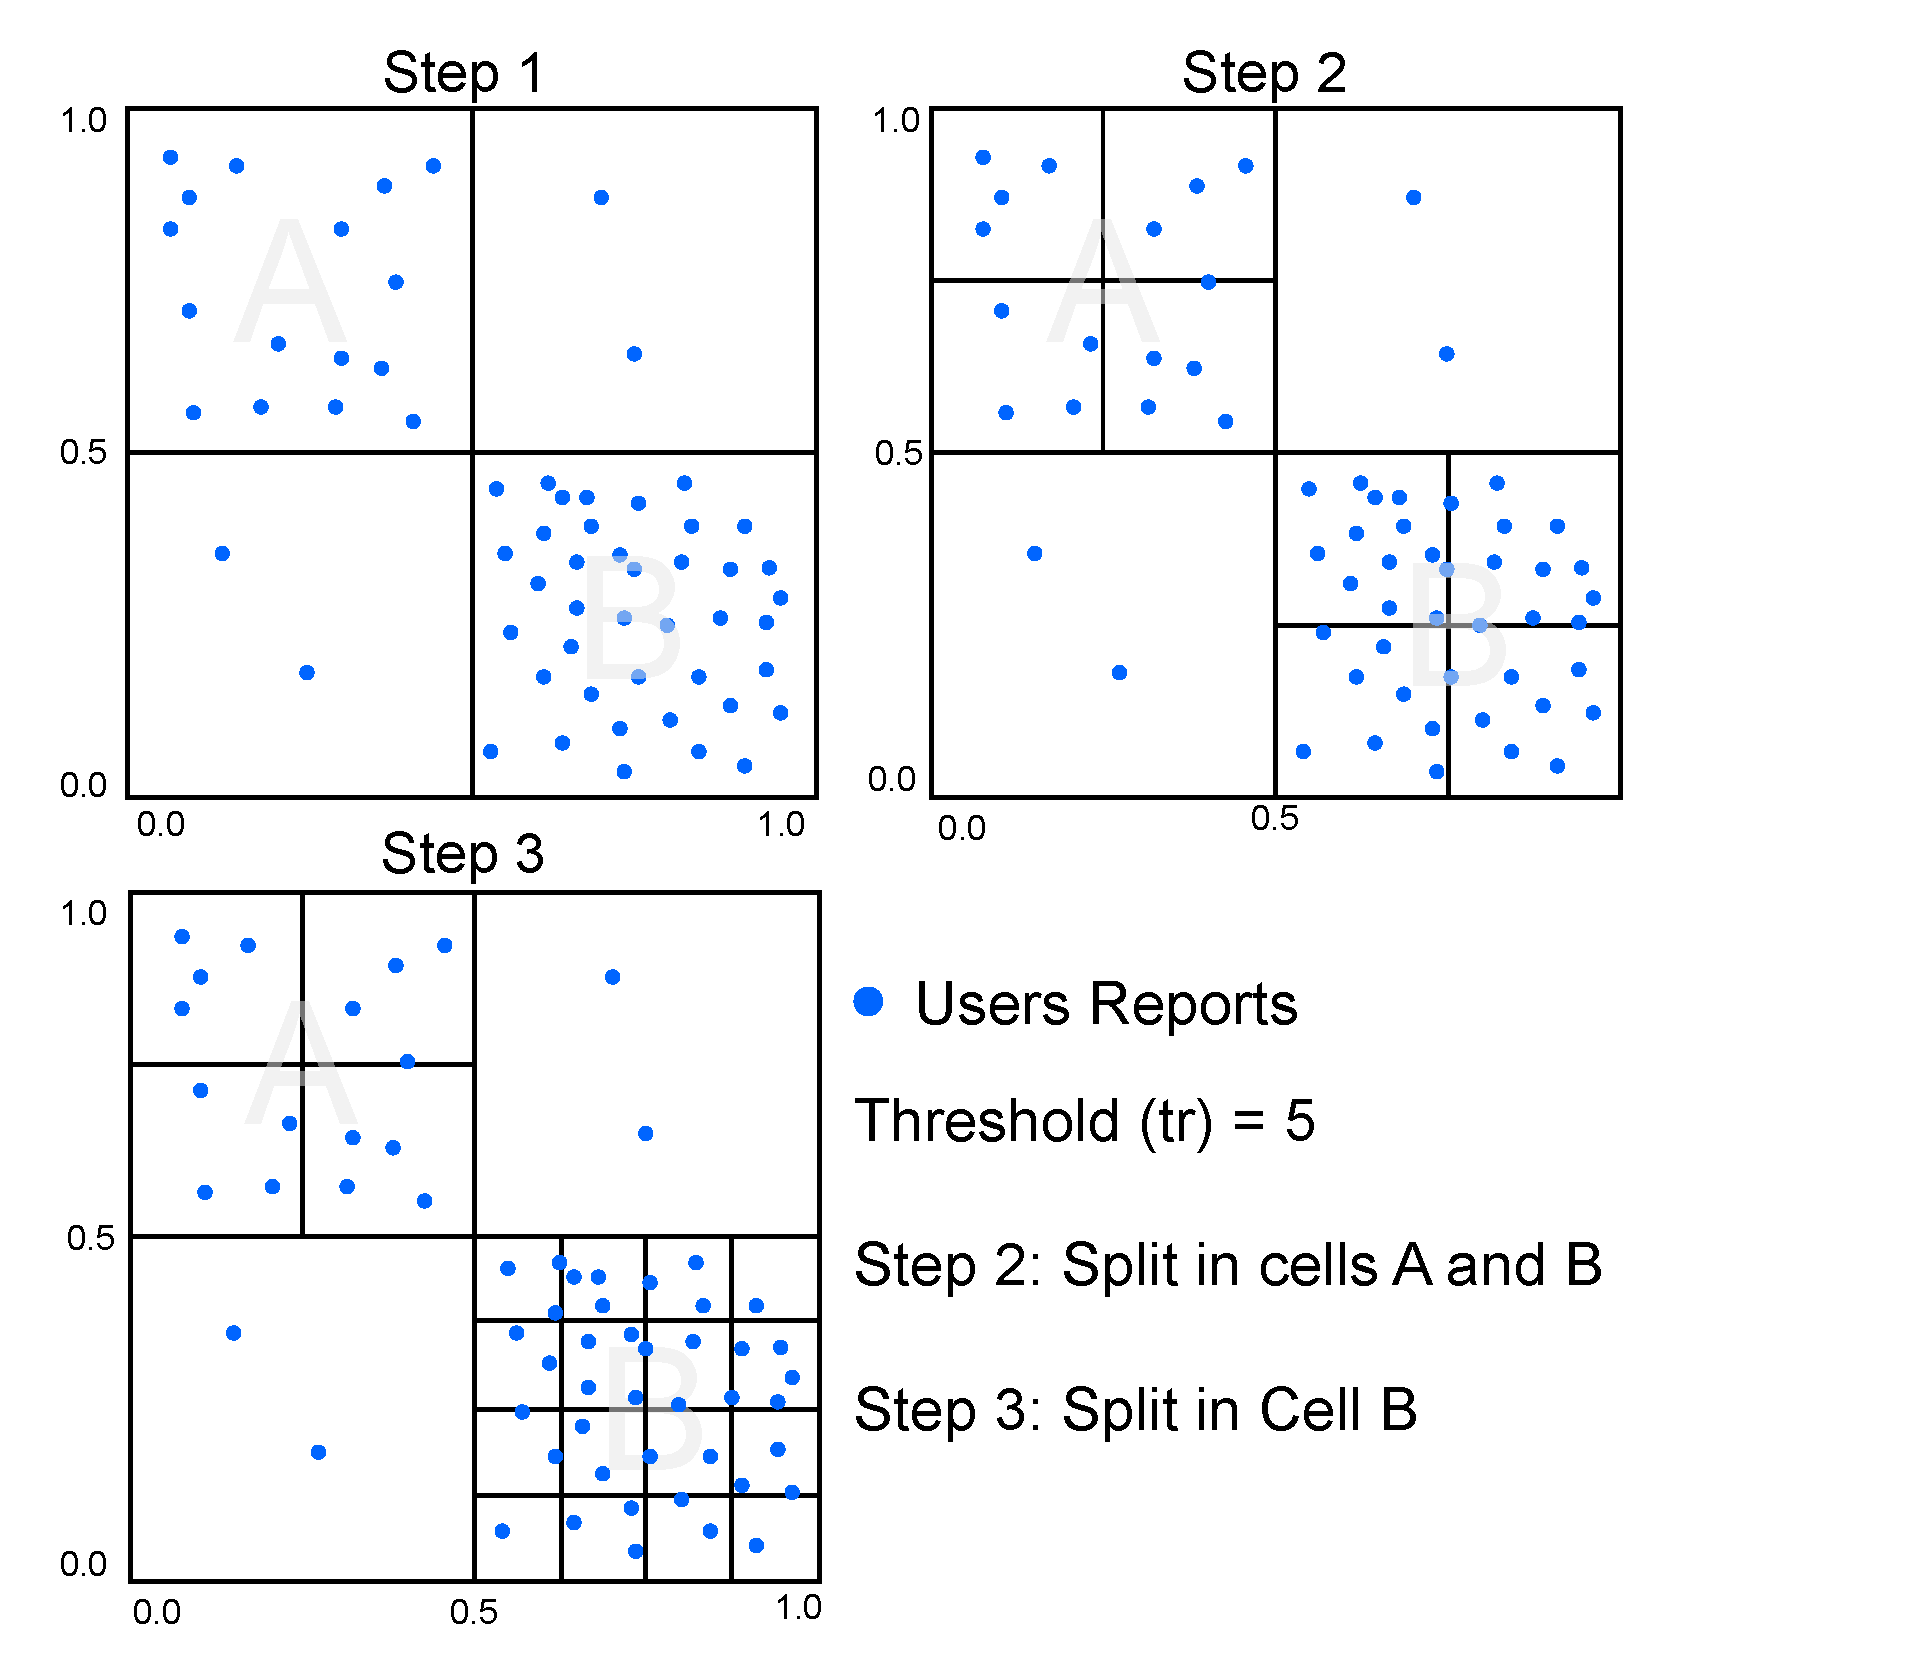
\includegraphics[width=\linewidth]{sections/figures/split_grid_seq_new.pdf}
    \caption{Illustration of the adaptive grid process: Cell A is split into four sub-cells after exceeding the threshold, and Cell B undergoes an additional split into sixteen sub-cells.
    }
    \label{fig:grid_adaptation}
\end{figure}

The first step in constructing the adaptive grid is to define the maximum allowable number of reports per cell, denoted as the cell threshold $tr$, which is determined by privacy requirements. Once the aggregator processes the users' reports for a specific timestamp $t$, it calculates the count $c_i$ of reports for each cell $g \in G$. Cells with report counts exceeding the threshold tr are recursively subdivided into four uniform cells, each occupying an equal portion of the original cell's spatial area. Subsequently, the count for each newly formed cell is assigned as one-quarter of the original cell count c, allowing the adaptive grid to dynamically adjust to areas of high report density by increasing granularity. This process is repeated until all cells satisfy the threshold tr. The complete algorithm for constructing the adaptive grid is detailed in Algorithm \ref{alg:recursive_adaptive_grid_creation}.

\begin{algorithm}[htb]
\small
\SetKwInOut{Input}{Input}
\SetKwInOut{Output}{Output}
\SetKwFunction{FGrid}{AdaptativeGrid}
\SetKwFunction{FSplit}{SplitCell}
\SetKwFunction{FMain}{Main}
\SetKwProg{Fn}{Function}{:}{}
\SetAlgoNoLine

\Input{Grid $G$, Estimated frequency for timestamp \( t \), Cell threshold \( tr \)}
\Output{Adaptive grid with updated cell counts}

\Fn{\FGrid($G$)}{
    % Process the frequency estimations to aggregate counts for each grid cell\;
    Calculate $\forall i\in G: c_i := \hat{f}_i$\;
    \For{each cell \( i \)}{
        SplitCell($\langle i, c_i\rangle$)\;
    }
}

\Fn{\FSplit($\langle i, c_i\rangle$)}{
    \If{\( c_i > tr \)}{
        Split cell \( i \) into four sub-cells of equal area\;
        \For{each sub-cell \( j \) of cell \( i \)}{
            Set count for sub-cell \( j \) to \( c_j = \frac{c_i}{4} \)\;
            \For{each cell \( i \)}{
                SplitCell($\langle i, c_i\rangle$)\;
                %Recursive call
            }
        }
    }
}
% \Return{Adaptive grid with updated cell counts}
\caption{Adaptive Grid Creation Algorithm}
\label{alg:recursive_adaptive_grid_creation}
\end{algorithm}
% 
Figure \ref{fig:grid_adaptation} illustrates the grid adaptation process. In the transition from Box 1 to Box 2, cells $A$ and $B$ are each split into four smaller cells. While cell $A$ reaches a count below the threshold $tr$, cell $B$ still exceeds the threshold, requiring an additional split in Box 3. As a result, all cells achieve a more balanced distribution of reports, ensuring a more uniform spatial representation. The time complexity of the adaptive grid creation is $\mathcal{O}(k \log n)$, where $k$ is the number of initial grid cells and $n$ is the number of user reports, reflecting the recursive subdivision of high-density cells.


\subsection{Frequency Estimator Framework}
\label{sec:fef}

ALOG comprises two main components: the users, who send encoded reports of their private locations, and the aggregator, who is responsible for collecting these reports and estimating the frequency of each grid cell. Beyond frequency estimation, the aggregator also contributes to generating and distributing the adaptive grid—a spatial representation that dynamically adjusts according to report density—to users. This adaptive grid enables refined spatial partitioning that is aligned with the population distribution, enhancing the precision of data collection and analysis.

Initially, the aggregator broadcasts a uniform grid accessible to all users, partitioning the reference space—such as a city—into square cells of equal size. On the user side, each user encodes their current location according to the grid provided by the aggregator, as detailed in Section \ref{sec:space_partition}. Utilizing a local differential privacy protocol, each user sends a noisy, obfuscated report of their location back to the aggregator. ALOG leverages the LOSUE protocol \ref{sec:losue}, which, following empirical analysis, has proven well-suited to this context; however, other longitudinal LDP protocols could also be employed.

Grid refinement is essential for reducing non-uniformity errors and improving data utility. However, evolving grids during anonymization can decrease memoization efficiency, leading to higher privacy budget consumption. This inefficiency arises because new cells are created with each new grid generated during the adaptation process. As a result, the previous canonical mapping of data to grid cells must be discarded, requiring the system to reinitialize the memoization for the newly created grid structure.

To mitigate this trade-off between budget consumption and grid adaptation, we propose a Grid Adaptation Window (GAW) mechanism. This mechanism ensures that grid adaptations occur only after every $w$ consecutive timestamps, after which the updated grid is broadcast to the users. Figure \ref{fig:window} illustrates the grid adaptation process with a window size of 2. Despite the use of GAW, the aggregator continues performing frequency estimations at each timestamp, ensuring continuous system monitoring and analysis. 

\begin{figure}[!ht]
    \centering
    \Description{GAW process}
    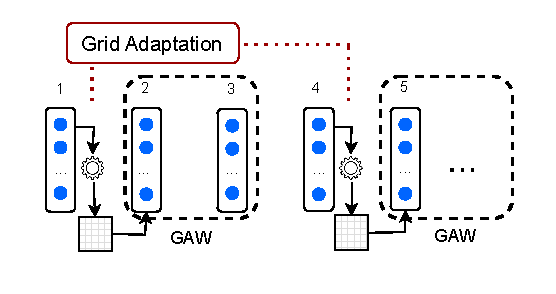
\includegraphics[width=0.8\linewidth]{sections/figures/gaw.pdf}
    \caption{GAW: Grid Adaptation Window mechanism with time window of size $w=2$}
    \label{fig:window}
\end{figure}

An additional benefit of the GAW is that it addresses situations where grid refinement is not always necessary. In some cases, the gain from refining the grid is not significant enough to justify the additional computational cost, as there may be little to no change between consecutive occurrences. In these situations, the GAW mechanism effectively reduces unnecessary grid adaptations, ensuring that system performance remains optimal without compromising the accuracy of the frequency oracles. The entire ALOG algorithm is detailed in Algorithm \ref{alg:alog_combined}.

% In the remainder of this section, we present a detailed exploration of the variations introduced by the proposed ALOG approach. The full ALOG algorithm is detailed in Algorithm \ref{alg:alog_combined}.


\begin{algorithm}[h]
\small
\SetKwInOut{Input}{Input}
\SetKwInOut{Output}{Output}
\SetAlgoNoLine

% User-side Algorithm
\textbf{User-side:} \\
\Input{$w$ \textit{(grid adaptation window)}}
\Output{Report $\hat{r}_i$}

\For{each timestamp $t$}{
    $l_i$ = Capture current location \\
    $G$ = Receive the Grid from Server\\
    $r_i$ = Encode($l_i$,$G$) \\
    $M$ = Initialize the Memoization Vector ($G$) \\

    $\hat{r}_i$ = LDP Protocol($r_i$, $G$, $M$)\;

    \If{\( t \% w == 0 \)}{
        $M$ = Initialize the Memoization Vector ($G$)\;
    }
}

% Server-side Algorithm
\textbf{Server-side:} \\
\Input{$tr$ \textit{(Cell Threshold)}, $w$ \textit{(grid adaptation window)}}
\Output{Adaptive grid, Frequency Estimations}

$G$ = Initialize the initial Grid\;

Process the reports to aggregate counts for each grid cell\;

\For{each timestamp $t$}{
    $R$ = Receive the reports for all users \\
    $F$ = Aggregate the reports to process the frequency estimation ($R$)\;
    \If{\( t \% w == 0 \)}{
        $G$ = Adaptive Grid Creation Algorithm ($G$, $F$, $tr$)\;
    }
}
\caption{ALOG Algorithm}
\label{alg:alog_combined}
\end{algorithm}

We propose three variations of the ALOG approach to determine the most effective solution for anonymizing user location reports in the context of grid refinement and data utility. The first variation, \textbf{ALOG-2R}, implements a two-round sanitization process designed to improve both grid refinement and the utility of the data. In the first round, each user $i$ anonymizes their location report using the initially provided uniform grid, allocating only a fraction of the available privacy budget to this step. For example, suppose a user $i$ has a true location at $(x_i, y_i)$, and the initially assigned grid cell is $g_0$. The user first encodes their location into the grid cell $g_0$ (e.g., by rounding their location to the nearest cell in the grid). The user then applies a Local Differential Privacy (LDP) protocol, utilizing a fraction of the total privacy budget to anonymize the encoded location. The resulting anonymized report, denoted as $\hat{r}_i$, is sent to the aggregator. This initial stage aims to provide a preliminary anonymized data sample to the aggregator.

Once the aggregator has collected the anonymized reports from all users, it proceeds to refine the spatial grid based on these reports. Specifically, the aggregator applies the Adaptive Grid Creation Algorithm (Algorithm \ref{alg:recursive_adaptive_grid_creation}) to construct a refined, adaptive grid that more accurately reflects the underlying data distribution. This adaptive grid is tailored to capture variations in the density of user locations, allowing for more precise spatial partitioning.

In the second round, the user $i$ now anonymizes their true location using the refined grid. For instance, if the user's true location $(x_i, y_i)$ falls in a newly created, smaller grid cell $g_1$ (which results from the adaptive grid refinement), the user will now encode their location into this smaller, more precise grid cell $g_1$. The user then applies the remaining portion of their privacy budget to anonymize the location in this refined grid cell, using the same LDP protocol as in the first stage. This refined anonymization ensures that the user's location is represented with higher precision according to the new adaptive grid. The anonymized report is then sent to the aggregator. After all users have submitted their second-round reports, the aggregator collects these updated anonymized reports and performs frequency estimation for the given timestamp. With grid refinement in the first stage and a more precise anonymization in the second stage, this two-stage process results in improved utility. By incorporating the adaptive grid refinement early on, ALOG-2R ensures that the data is processed with an optimized spatial partitioning, leading to more accurate frequency estimations while maintaining a strong privacy guarantee.

Alternatively, \textbf{ALOG-1R-a} (One-Round Sanitization — Adaptive) and \textbf{ALOG-1R-b} (One-Round Sanitization — Baseline) utilize a single-round sanitization process. In both variations, users initially report perturbed data using a uniform grid, and the adaptive grid is applied only in subsequent reports. The key distinction between ALOG-1R-a and ALOG-1R-b lies in the choice of the base grid used during the adaptation process.


In ALOG-1R-a, the base grid used for adaptation is not static. Instead, the grid from the previous adaptation step serves as the input for the Adaptive Grid Creation Algorithm. This allows for incremental refinements over time, where the grid is continuously adjusted to reflect the evolving spatial patterns of user locations. For instance, suppose in the first timestamp, a user $i$ has a true location at $(x_i, y_i)$, which initially maps to a grid cell $g_0$. After anonymizing the location using LDP and sending the anonymized data to the aggregator, the adaptive grid is refined based on the collected reports. When the user submits their report in the next timestamp, the adaptive grid generated from the prior stage is used as the base grid for further refinement. If the user's true location $(x_i, y_i)$ now falls into a more precise, smaller grid cell $g_1$ in this updated grid, the user will anonymize their location based on this refined grid, improving the accuracy of the spatial partitioning with each adaptation step. This dynamic approach allows the system to adapt to changing patterns in user data, improving the overall utility while maintaining privacy.

Conversely, in ALOG-1R-b, the algorithm takes a different approach. Here, the adaptive grid is reset at every adaptation step, and the algorithm consistently uses the default uniform grid as the base grid for every iteration of the grid refinement process. In each adaptation step, the algorithm ignores any previous refinements and starts from the uniform grid, applying the Adaptive Grid Creation Algorithm as if it were the first round of processing. For example, a user $i$'s true location $(x_i, y_i)$ is first mapped to a grid cell $g_0$ of the uniform grid. After anonymizing their location using LDP and sending the anonymized report to the aggregator, the grid is adapted based on the collected data. This new adaptive grid will be used in the next timestamp for users to anonymize their location, but the grid is discarded for the next adaptation process. When the user submits their second report, the algorithm again uses the uniform grid as the base for the refinement, disregarding the previous adaptation. This results in a stable reference framework for the grid adaptation process, which may be more predictable but does not account for changes in user spatial distributions over time.


% \begin{figure}[!ht]
%     \centering
%     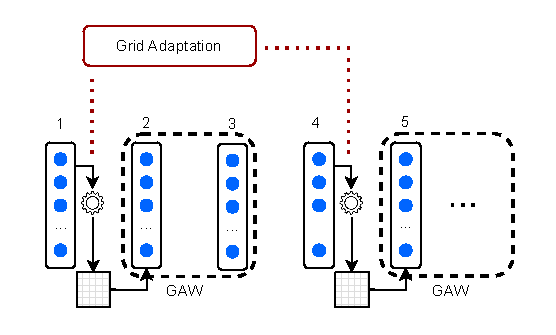
\includegraphics[width=0.8\linewidth]{sections/figures/ldpFE_trajectory-GAW.pdf}
%     \caption{GAW: Grid Adaptation Window mechanism with time window of size $w=2$}
%     \label{fig:window}
% \end{figure}


% \begin{table}[h!]
% \centering
% \caption{ALOG Variations}
% \footnotesize
% \begin{tabular}{l|c|c}
% % \begin{tabular}{ccc}
% \toprule
% \textbf{Approach} & \textbf{Rounds of Sanitization} & \textbf{Base Grid for Adaptation} \\
% \midrule
% ALOG-2R & Two-round & Previous Grid \\
% ALOG-1R-a & Single round & Previous Grid \\
% ALOG-1R-b & Single round & Uniform Grid \\
% \bottomrule
% \end{tabular}
% \end{table}

\begin{figure}[!ht]
    \centering
    \Description{Aloq workflow}
    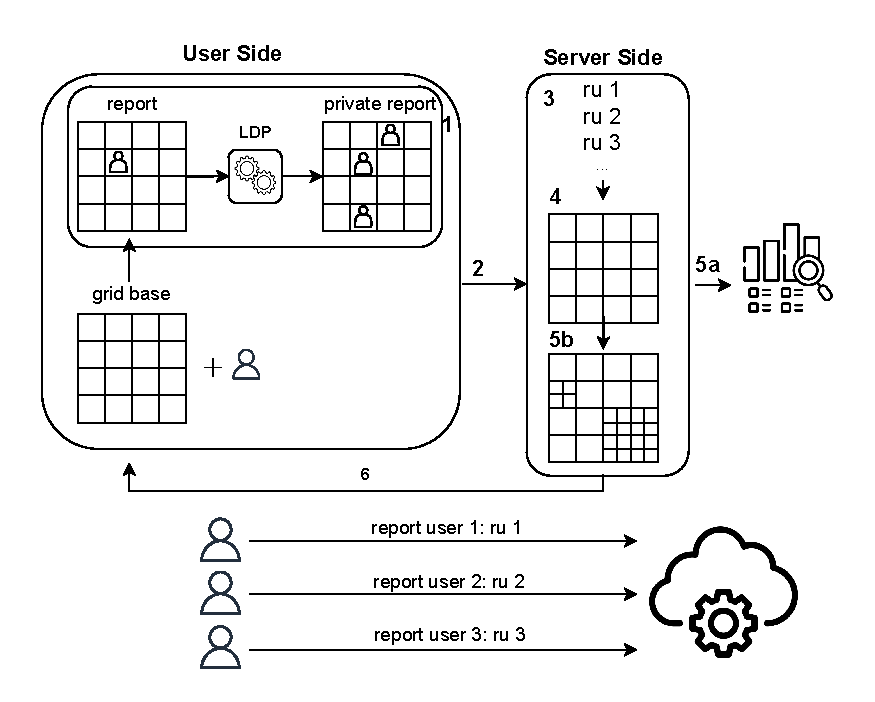
\includegraphics[width=0.8\linewidth]{sections/figures/alog_fe.pdf}
    \caption{ALOG Workflow - Step 1: Users sanitize their own reports. Step 2: Send the sanitized reports to the aggregator. Step 3: Aggregate received reports. Step 4: Process count for each cell. Step 5a: Perform frequency estimation. Step 5b: Grid adaptation to refine spatial granularity. Step 6: Broadcast the new Grid}

    \label{fig:alog_wf}
\end{figure}

The workflow of ALOG is illustrated in Figure \ref{fig:alog_wf}. The process begins with Step 1, performed on the user side, where each user encodes their location using the current base grid provided by the aggregator. This grid could either be the initial uniform grid (for ALOG-1R-b) or the refined grid from the previous moment (for ALOG-1R-a and ALOG-2R). The user applies a Local Differential Privacy (LDP) protocol to anonymize the location report in all approaches. Once anonymized, the report is transmitted securely to the aggregator, completing Step 2.

In Step 3, the aggregator collects all received reports. Step 4 follows, where the aggregator counts the occurrences within each grid cell to estimate the spatial distribution of user locations. Step 5a is executed at every timestamp, regardless of the approach. In this step, the aggregator publishes the estimated spatial distribution for each grid cell based on the received reports. This frequency estimation is critical for maintaining real-time monitoring of the data. The distinction arises when a Grid Adaptation Window (GAW) concludes. The GAW mechanism, primarily used in ALOG-2R and ALOG-1R-a, allows the grid adaptation process to occur only after a predefined number of timestamps (denoted as w). When this window ends, Step 5b is triggered. During Step 5b, the grid cells are adjusted based on report density. This refinement aims to enhance spatial resolution and precision, tailoring the grid to represent the underlying distribution of user locations better. This adjustment will occur as follows for each approach:
% 
\begin{itemize}
    \setlength{\parskip}{0pt}
    \setlength{\itemsep}{0pt plus 1pt}
    \item ALOG-2R: Grid refinement occurs after every w timestamp, allowing for dynamic, incremental adaptations. This means that after each window of w timestamps, the aggregator adapts the grid based on the spatial distribution observed in those reports.
    \item ALOG-1R-a: Similarly, the grid is adapted after every w timestamps, but in this approach, the refinement is based on the previously adapted grid. The grid evolves incrementally, becoming more precise with each new adaptation.
    \item ALOG-1R-b: In this approach, even when the GAW ends, the grid is reset to the initial uniform grid at every adaptation step, discarding any previous refinements. This provides a stable reference framework but does not consider previous grid adaptations.
\end{itemize}
% 
Finally, in Step 6, the aggregator broadcasts the refined grid back to the users. This ensures that users always work with an up-to-date spatial representation of the data. The users then continue the process of encoding, anonymizing, and sending reports based on the latest grid, ensuring that the system adapts to real-time patterns. \looseness=-1

This entire workflow is designed to repeat iteratively, maintaining a dynamic balance between spatial precision and privacy guarantees. The GAW ensures that grid adaptations occur controlled, reducing unnecessary overhead, while the different approaches (ALOG-1R-a, ALOG-1R-b, and ALOG-2R) offer flexibility depending on the need for stability versus dynamic adaptation.

On the client side, the ALOG algorithm \ref{alg:alog_combined} has a per-timestamp time and space complexity of $\mathcal{O}(k)$, where $k$ is the number of grid cells. This cost stems from encoding the location as a unary vector and applying the LDP mechanism. The time complexity of the ALOG algorithm on the server side, assuming a one-round approach, can be described in terms of the number of grid cells $k$, the number of user reports $n$, and the grid adaptation window size $w$. For each timestamp, the server processes $n$ reports and performs frequency estimation over $k$ cells, leading to a per-timestamp cost of $\mathcal{O}$($nk$). Every $w$ timestamps, the adaptive grid is updated using a recursive algorithm, whose worst-case cost is $\mathcal{O}(k \log n)$ due to cell subdivisions based on report density. Thus, over a time horizon $T$, the amortized server-side complexity becomes 
$\mathcal{O}$($Tnk + wTk\log n$), balancing continuous frequency estimation with periodic grid refinement.

\subsection{Privacy and Utility Analysis}
\label{sec:privacy}

In our approach, we employ LDP to protect user privacy while estimating the frequency of each grid cell in a spatial domain. Each user perturbs their location data locally before transmitting it to a centralized aggregator. This is done using the LOSUE protocol, as Section \ref{sec:losue} explains.

At each timestamp, ALOG uses at most a privacy budget of $\epsilon_\infty$, even ALOG-2R. In the case of ALOG-2R, the $\epsilon_\infty$ is divided across two stages: a fraction of $\epsilon_\infty$ is spent in the first stage, and the remaining fraction is applied in the second stage. Like other data collection models, whether using adaptive grids or not, ALOG consumes a privacy budget of $\epsilon_\infty$ for a single report, which is the single report's upper bound. 

Proposition \ref{prop:alogdp} provides a pessimistic worst-case privacy guarantee for our approach. Nevertheless, our experiments demonstrate that ALOG achieves Pareto efficiency -- a state where no further improvement can be made to one objective (e.g., utility) without degrading another (e.g., privacy) -- even with a slightly higher theoretical privacy budget than competing methods.
\newcommand{\budget}{\eta \epsilon_\infty}

\begin{proposition}[ALOG's Privacy Guarantee]
    The ALOG algorithm guarantees, in the worst case,  
    \(\budget\)-local differential privacy, where: \looseness=-1
        \(\eta = \left( \sum_{r=0}^R (k - \bar{k}) \cdot 4^r + \bar{k} \right)\),
        \( \bar{k} \) is the number of initial grid cells satisfying the threshold condition,
        \( R = \left\lceil \log_4 \frac{|U|}{tr} \right\rceil \) is the maximum recursion depth of the Algorithm \ref{alg:recursive_adaptive_grid_creation},
        \( \epsilon_\infty \) is the per-report privacy budget under \( \Psi \), the underlying LDP mechanism.  
    \label{prop:alogdp}
\end{proposition}
\begin{proof}
    At initialization, the grid contains \( k \) cells, of which \( \bar{k} \) satisfy the threshold \( tr \). The remaining \( k - \bar{k} \) cells are recursively split (at most \( R \) times) until all subcells meet \( tr \), as formalized in Algorithm \ref{alg:recursive_adaptive_grid_creation}. \looseness=-1
    For recursion level \( r \in [0, R] \), the grid contains \( (k - \bar{k}) \cdot 4^r + \bar{k} \) cells. Summing over all levels, the \textit{total cumulative cell count} is:  
    \( 
    \sum_{r=0}^R \left( (k - \bar{k}) \cdot 4^r + \bar{k} \right).  
    \) 
    Since each user’s location report is privatized via \( \Psi \) (an \( \epsilon_\infty \)-LDP protocol), the \textit{longitudinal privacy cost} of ALOG, accounting for adaptive grid construction and repeated reporting, is bounded by the worst-case total cell count multiplied by \( \epsilon_\infty \). This holds because:
    \begin{enumerate}
        \item \textit{User-side perturbation}: Each report is independently \( \epsilon_\infty \)-LDP.
        \item \textit{Aggregator-side adaptation}: The grid’s dynamic refinement does not access raw data, relying only on privatized counts.
    \end{enumerate}
    The total cumulative cell count reflects the worst-case scenario where Algorithm \ref{alg:recursive_adaptive_grid_creation} exhausts all possible recursions. Each cell is sanitized only once during the longitudinal process by employing memoization in the LDP protocol. Thus, since the upper bound on cell count is \( \eta \), the maximum number of sanitizations is precisely the cumulative cell count.
    As each report is independently \( \epsilon_\infty \)-LDP and there are at most \(\eta\) cells in the grid, our proposed algorithm is \(\budget\)-local differentially private.
\end{proof}


In ALOG, both the frequency estimation (Section \ref{sec:freq_estimator}) and grid adaptation (Section \ref{sec:adaptative_grid}) processes operate on the perturbed reports, ensuring that individual location data remains protected. As Proposition \ref{prop:seq_processing} states, any function applied to the output of an $\epsilon$-LDP mechanism preserves $\epsilon$-LDP privacy guarantees, meaning that the privacy established by the initial LDP perturbation is maintained throughout these post-processing steps without introducing additional privacy risks.

The granularity of the initial grid used in LDP significantly impacts data sensitivity and privacy preservation. This relationship is analyzed through variance, a key measure of frequency estimate accuracy and reliability. The variance of LDP protocols is inversely proportional to the number of times a value \(v_i\) has been reported \cite{arcolezi2022frequency}, meaning that higher variance indicates greater uncertainty and error in estimates. In comparison, lower variance suggests more accurate results. Fine-grained grids yield fewer reports per cell in low-density areas, increasing variance and making estimates less reliable. Conversely, in high-density areas, fine-grained grids can maintain utility without compromising privacy, as the number of reports per cell remains high, reducing variance.

ALOG directly addresses the variance problem by using coarser grids in low-density areas, increasing reports per cell and decreasing variance. ALOG refines the grid in high-density areas to maintain utility, and the higher density helps control variance. Due to this adaptive behavior, ALOG's grids tend to keep the density between cells close to uniformity, further enhancing the accuracy of estimates while preserving privacy.

When handling longitudinal data, ALOG mitigates privacy loss through the Grid Adaptation Window (GAW). By regulating the frequency of grid adjustments, the GAW ensures that the grid adapts only after every \(w\) timestamps, limiting the reinitialization of memorization, which is a process that consumes the privacy budget. This mechanism balances the utility gains offered by dynamic grid adaptation and the potential increase in privacy loss resulting from frequent re-randomization, thus maintaining privacy protection while enhancing utility.
\section{Experimental Evaluation}
\label{sec:exp_evaluation}
In this section, we present the experiments conducted to empirically demonstrate that our approach not only achieves higher utility but also maintains a stronger level of privacy compared to traditional local differential privacy (LDP) protocols such as RAPPOR (Section \ref{sec:rappor}), L-OSUE (Section \ref{sec:losue}), and LOLOHA (Section \ref{sec:loloha}). We implemented our solution in Python, including our partitioning strategy and protocols. \looseness=-1
% 
\subsection{Experimental Setup}
We evaluate our approach using two synthetic datasets created for this study and two real-world mobility datasets. The synthetic datasets simulate user movement within a 100 km$^2$ area and allow us to assess behavior under contrasting spatial distributions.  
\begin{itemize}
    \item \textbf{S1}: Users are distributed uniformly across the region.
    \item \textbf{S2}: Users follow a normal distribution centered in the region.
\end{itemize}

Each synthetic dataset simulates 10,000 users moving at a constant speed of 40 km/h, generating one location report per minute over 40 timestamps. Locations are constrained by the speed to ensure realistic trajectories.

The \textbf{GeoLife} dataset\footnote{\url{https://www.microsoft.com/en-us/download/details.aspx?id=52367}} contains GPS trajectories from 183 users in Beijing. We extracted 6,261 trajectories of 20 timestamps each.  
The \textbf{Porto} dataset\footnote{\url{https://www.kaggle.com/datasets/crailtap/taxi-trajectory?select=train.csv}} comprises data from 442 taxis in Porto, Portugal. We selected 10,000 trajectories, also with 20 timestamps. Table~\ref{tab:datasets} summarizes all datasets. 

We acknowledge the use of only two real-world datasets, a limitation imposed by the scarce availability of longitudinal datasets with precise coordinate data — a key requirement for our analysis. Nevertheless, the selected datasets offer meaningful and representative insights. \looseness=-1
% 
\begin{table}[tb]
\centering
\caption{Summary of Datasets Used in the Experiments}
% \scriptsize
\begin{tabular}{l|c|c|c}
\toprule
\textbf{Dataset} & \textbf{Type} & \textbf{Distribution} & \textbf{\#Trajectories} \\
\midrule
S1 & Synthetic & Uniform & 10,000  \\
S2 & Synthetic & Normal & 10,000  \\
GeoLife & Real-world & Real-world & 6,281  \\
Porto & Real-world & Real-world & 10,000  \\
\bottomrule
\end{tabular}
\label{tab:datasets}
\end{table}
% 
For each dataset, we simulate users submitting anonymized location reports using longitudinal LDP protocols. These reports are used to estimate cell frequencies over a uniform grid. We compare these results with those obtained using ALOG's three variations (ALOG-2R, ALOG-1R-a, and ALOG-1R-b) under identical conditions. \looseness=-1

\textit{Data Utility:}  
To assess utility, we compute the \textbf{Root Mean Squared Error (RMSE)} between the true and estimated frequency distributions over time. Let \( F_i = \{f_0, \dots, f_{|G_i|}\} \) and \( \hat{F}_i = \{\hat{f}_0, \dots, \hat{f}_{|G_i|}\} \) denote the true and estimated frequencies at timestamp \( t_i \). The utility error is defined as:
% 
\begin{equation}
\small
\label{eq:utility_error}
\text{Utility Error} = \frac{1}{|T|} \sum_{i=1}^{|T|} \sqrt{ \frac{1}{|G_i|} \sum_{j=0}^{|G_i|-1} (f_j - \hat{f}_j)^2 }
\end{equation}
% 
This metric captures the accuracy of frequency estimates over time and across different spatial distributions.

% \textit{Budget Consumption:}  
% We also evaluate the \textbf{privacy budget} consumption of each method. For each timestamp \( t_i \), the budget consumed is at most \( \epsilon_\infty \) during anonymization. The total budget is:

% \[
% \text{Total Budget Consumption} = \sum_{i=1}^{|T|} \epsilon_\infty
% \]

% We report the average total budget per user to capture the cumulative privacy cost across the experiment.

\textit{Budget Consumption:}  
We also evaluate the \textbf{privacy budget} consumption of each method. For each timestamp \( t_i \), the budget consumed is at most \( \epsilon_\infty \) during anonymization. The total budget consumption is: $\sum_{i=1}^{|T|} \epsilon_\infty$. We report the average total budget per user to capture the cumulative privacy cost across the experiment.



\subsection{Results}

\paragraph{Grid Granularity x Utility:}first, we analyze the adjustment of grid granularity, which is a key aspect of the proposed adaptive longitudinal grid framework. Specifically, we compare methods using static uniform grids with ALOG, starting from the same initial grid granularity. The relationship between grid granularity and data utility is central to understanding how the system adapts to different data distributions while balancing privacy constraints.


\definecolor{sn1}{rgb}{0.00392156862745098, 0.45098039215686275, 0.6980392156862745}
\definecolor{sn2}{rgb}{0.8705882352941177, 0.5607843137254902, 0.0196078431372549}
\definecolor{sn3}{rgb}{0.00784313725490196, 0.6196078431372549, 0.45098039215686275}
\definecolor{sn4}{rgb}{0.8352941176470589, 0.3686274509803922, 0.0}
\definecolor{sn5}{rgb}{0.8, 0.47058823529411764, 0.7372549019607844}
\definecolor{sn6}{rgb}{0.792156862745098, 0.5686274509803921, 0.3803921568627451}

\begin{figure}[tb] 
    \centering
    \Description{Granularity Plots}
    \begin{tikzpicture}
        \begin{axis}[
        hide axis,
        xmin=0, xmax=1,
        ymin=0, ymax=1,
        legend style={
            draw=none,
            inner sep=0,outer sep=0,
            column sep=.5ex, % Adjust spacing between columns
            legend columns=3, % Number of legend items per row
            at={(0.5,0)}, % Position legend below the axis
            anchor=south
        },
        width=\columnwidth % Fit within one column
        ]
            % ALOG-1R-a: diagonal lines pattern
            \addplot[
            pattern=north east lines,
            pattern color=sn1,
            area legend
            ] coordinates {(0,0)};
            \addlegendentry{ALOG-1R-a}
    
            % ALOG-1R-b: crosshatch pattern
            \addplot[pattern=north west lines, pattern color=sn2, area legend] 
                coordinates {(0,0)};
            \addlegendentry{ALOG-1R-b}
    
            % ALOG-2R: grid pattern
            \addplot[pattern=vertical lines, pattern color=sn3, area legend] 
                coordinates {(0,0)};
            \addlegendentry{ALOG-2R}
    
            % RAPPOR: solid red color with no pattern
            \addplot[fill=black, fill=sn6, draw=none, area legend] 
                coordinates {(0,0)};
            \addlegendentry{RAPPOR}
            
            % LOSUE: diagonal crosshatch pattern
            \addplot[pattern=crosshatch, pattern color=sn5, area legend] 
                coordinates {(0,0)};
            \addlegendentry{LOSUE}
    
            % LOLOHA: horizontal lines pattern
            \addplot[pattern=horizontal lines, pattern color=sn4, area         legend] 
                 coordinates {(0,0)};
            \addlegendentry{LOLOHA}
        \end{axis}
    \end{tikzpicture}

    \centering
    % First sequence
    \begin{subfigure}{0.49\textwidth} % Adjust subfigure size to fit single column
        \centering
        \begin{minipage}{0.80\textwidth}
            \centering
            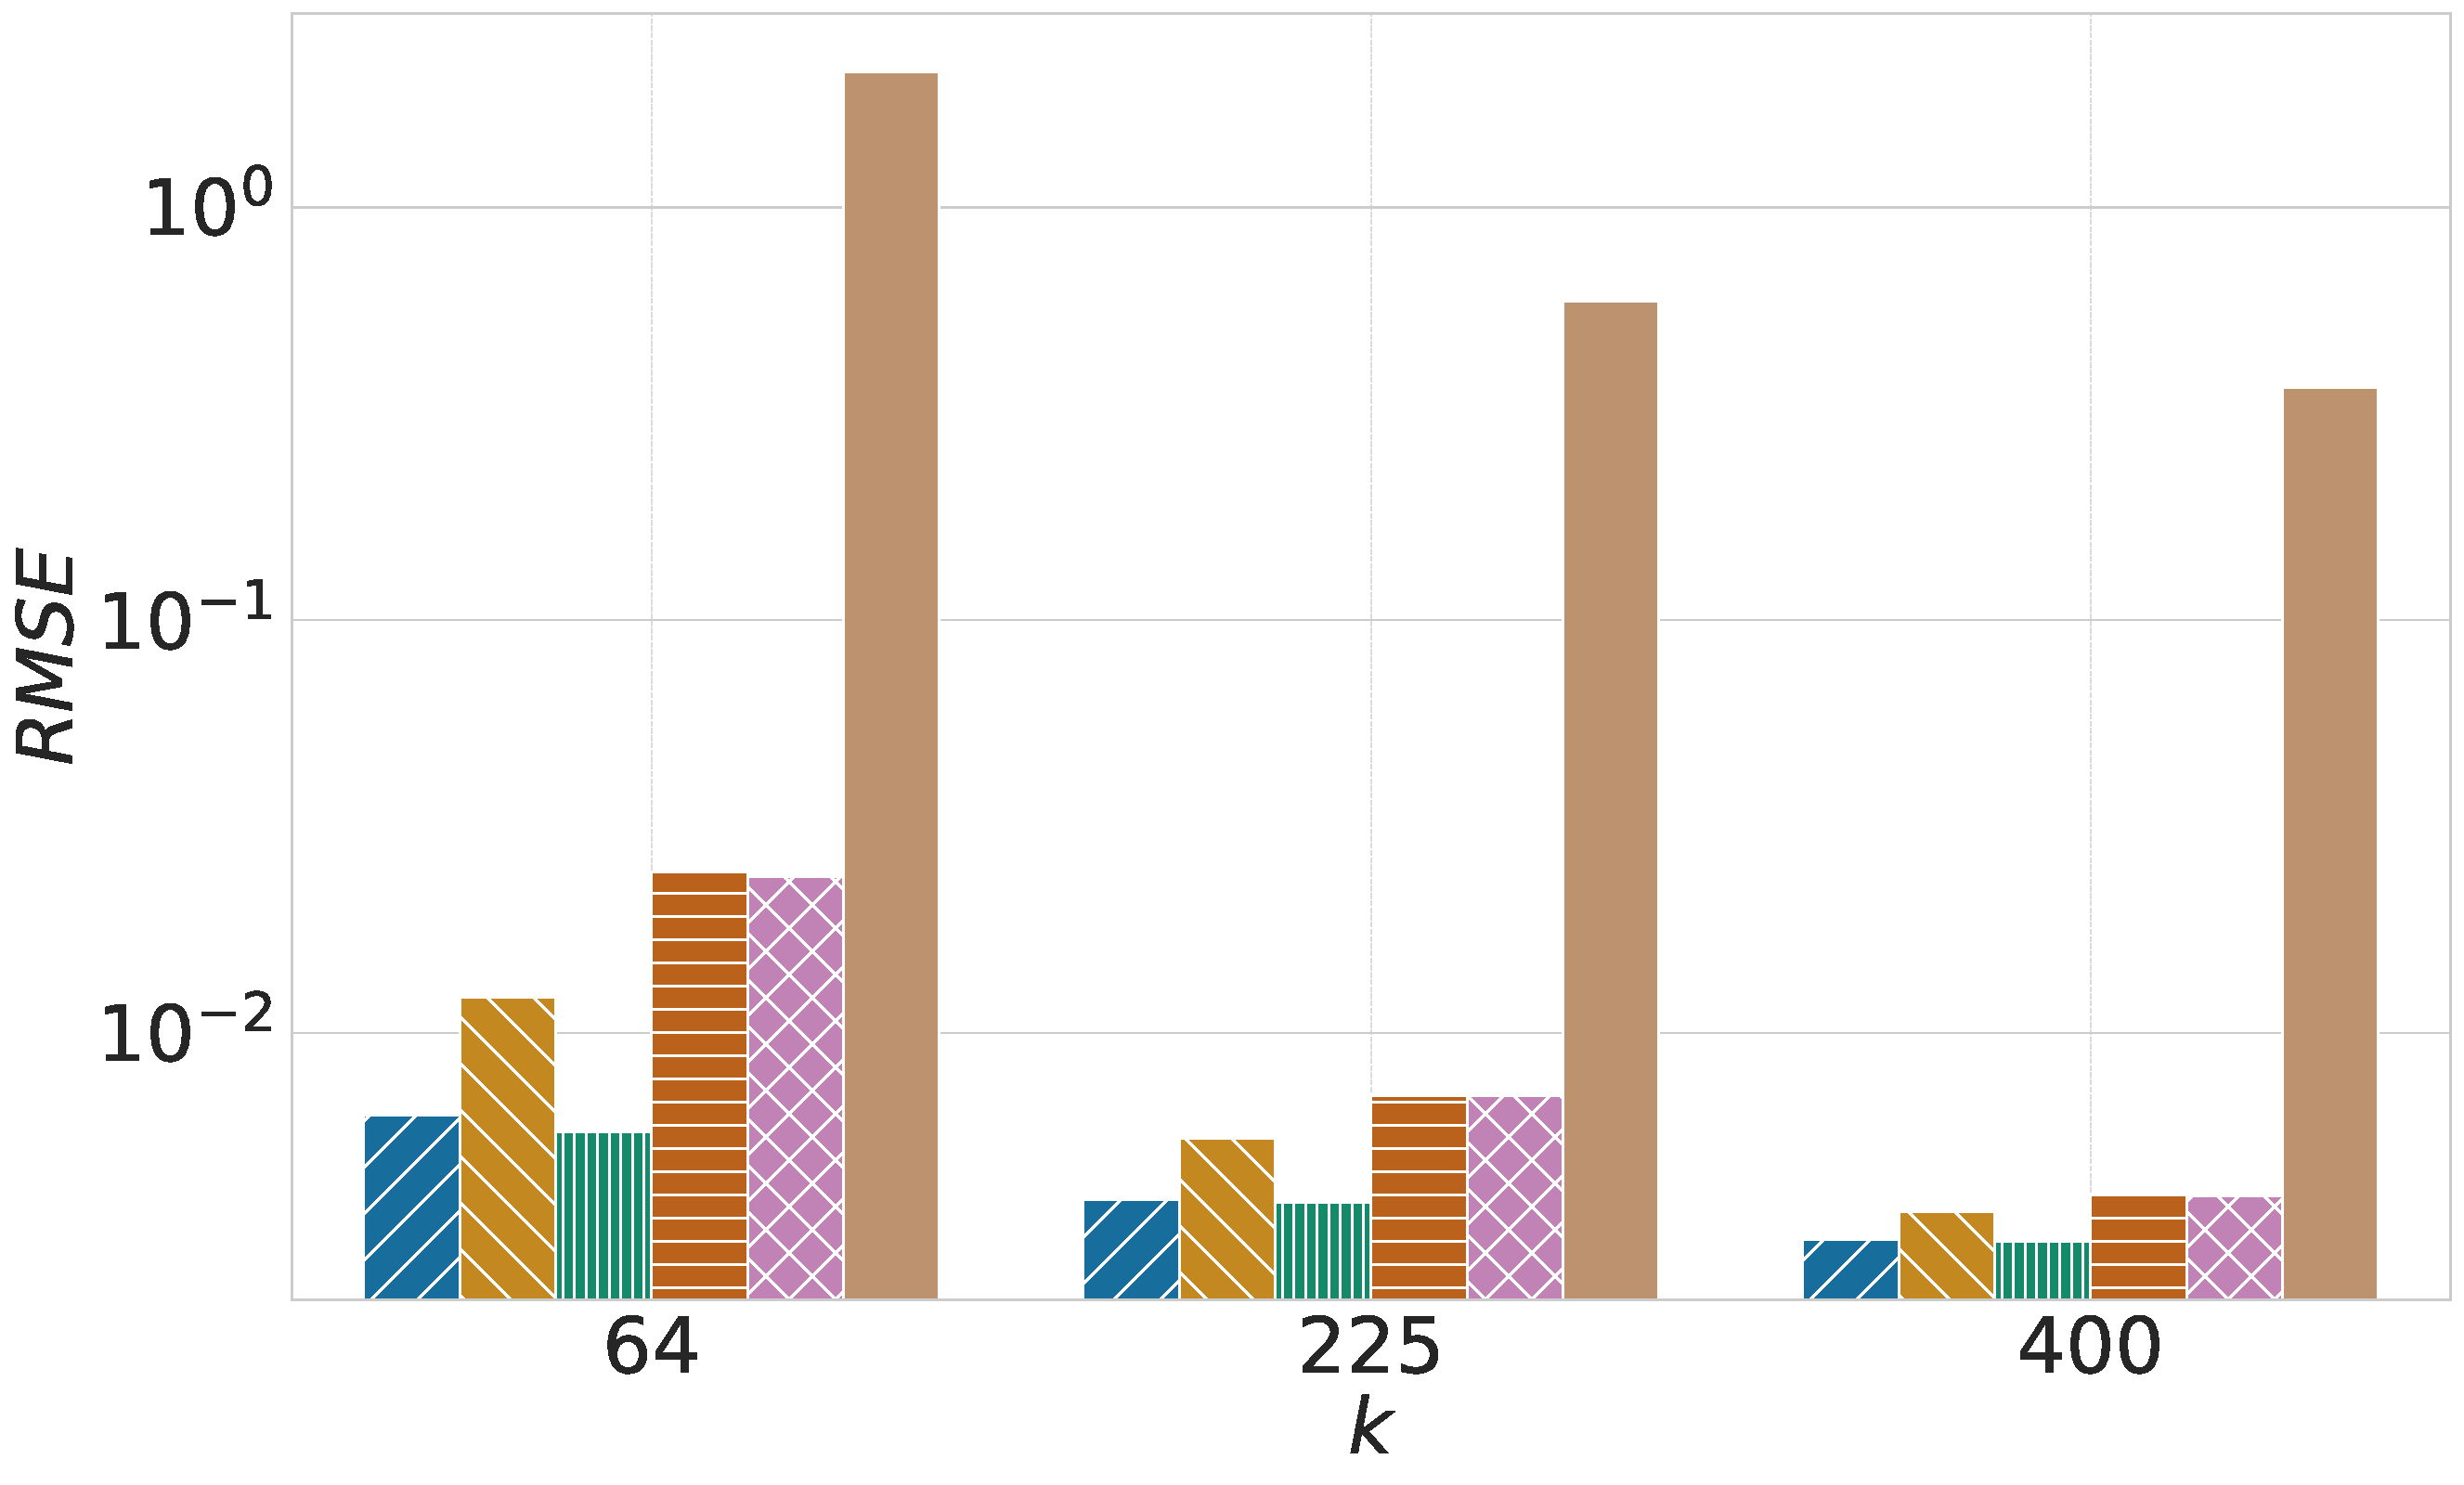
\includegraphics[width=\linewidth]{sections/figures/K_RMSE_BAR/rmse_compare_0.1_grid_avg_barchart_uniform.pdf}
            \caption{S1 with $\epsilon_{\infty}=0.1$}        
            \label{fig:granularity_s1}
        \end{minipage}
        \hfill
        \begin{minipage}{0.80\textwidth}
            \centering
            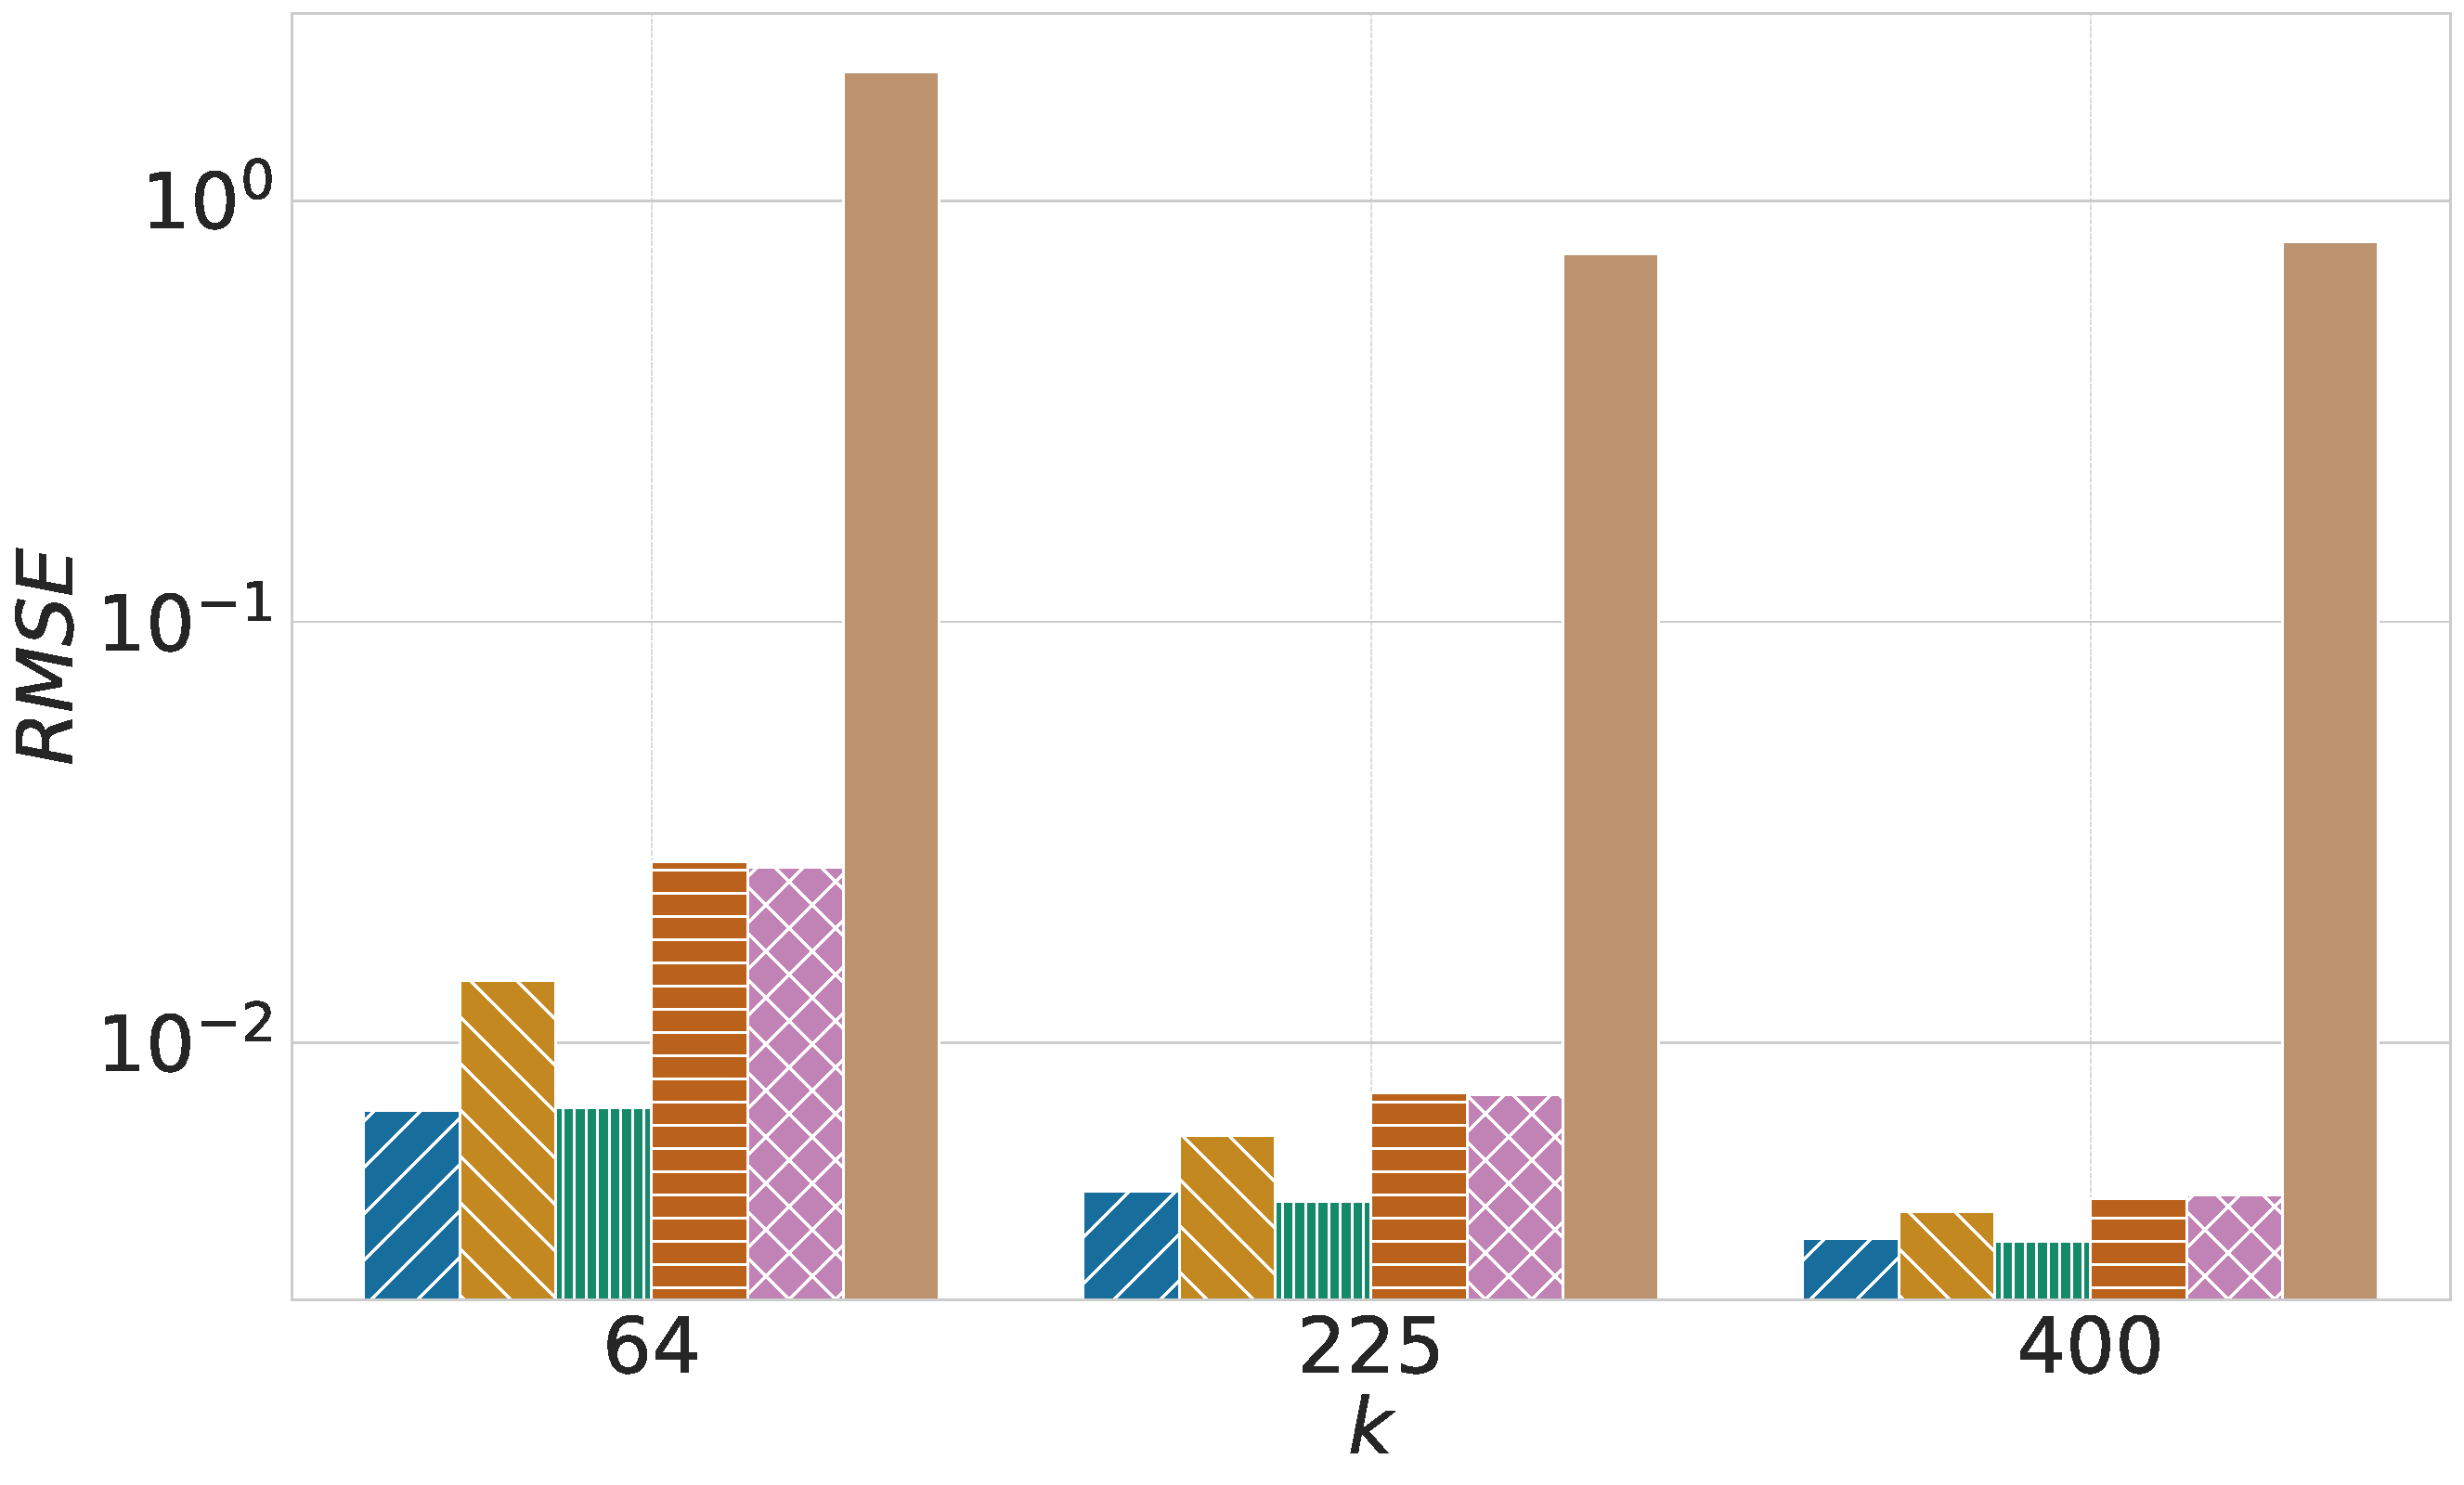
\includegraphics[width=\linewidth]{sections/figures/K_RMSE_BAR/rmse_compare_0.1_grid_avg_barchart_normal.pdf}
            \caption{S2 with $\epsilon_{\infty}=0.1$}
            \label{fig:granularity_s2}
        \end{minipage}
        \label{fig:sequence1}
    \end{subfigure}
    
    
    % Second sequence
    \begin{subfigure}{0.49\textwidth} % Adjust subfigure size to fit single column
        \centering
        \begin{minipage}{0.8\textwidth}
            \centering
            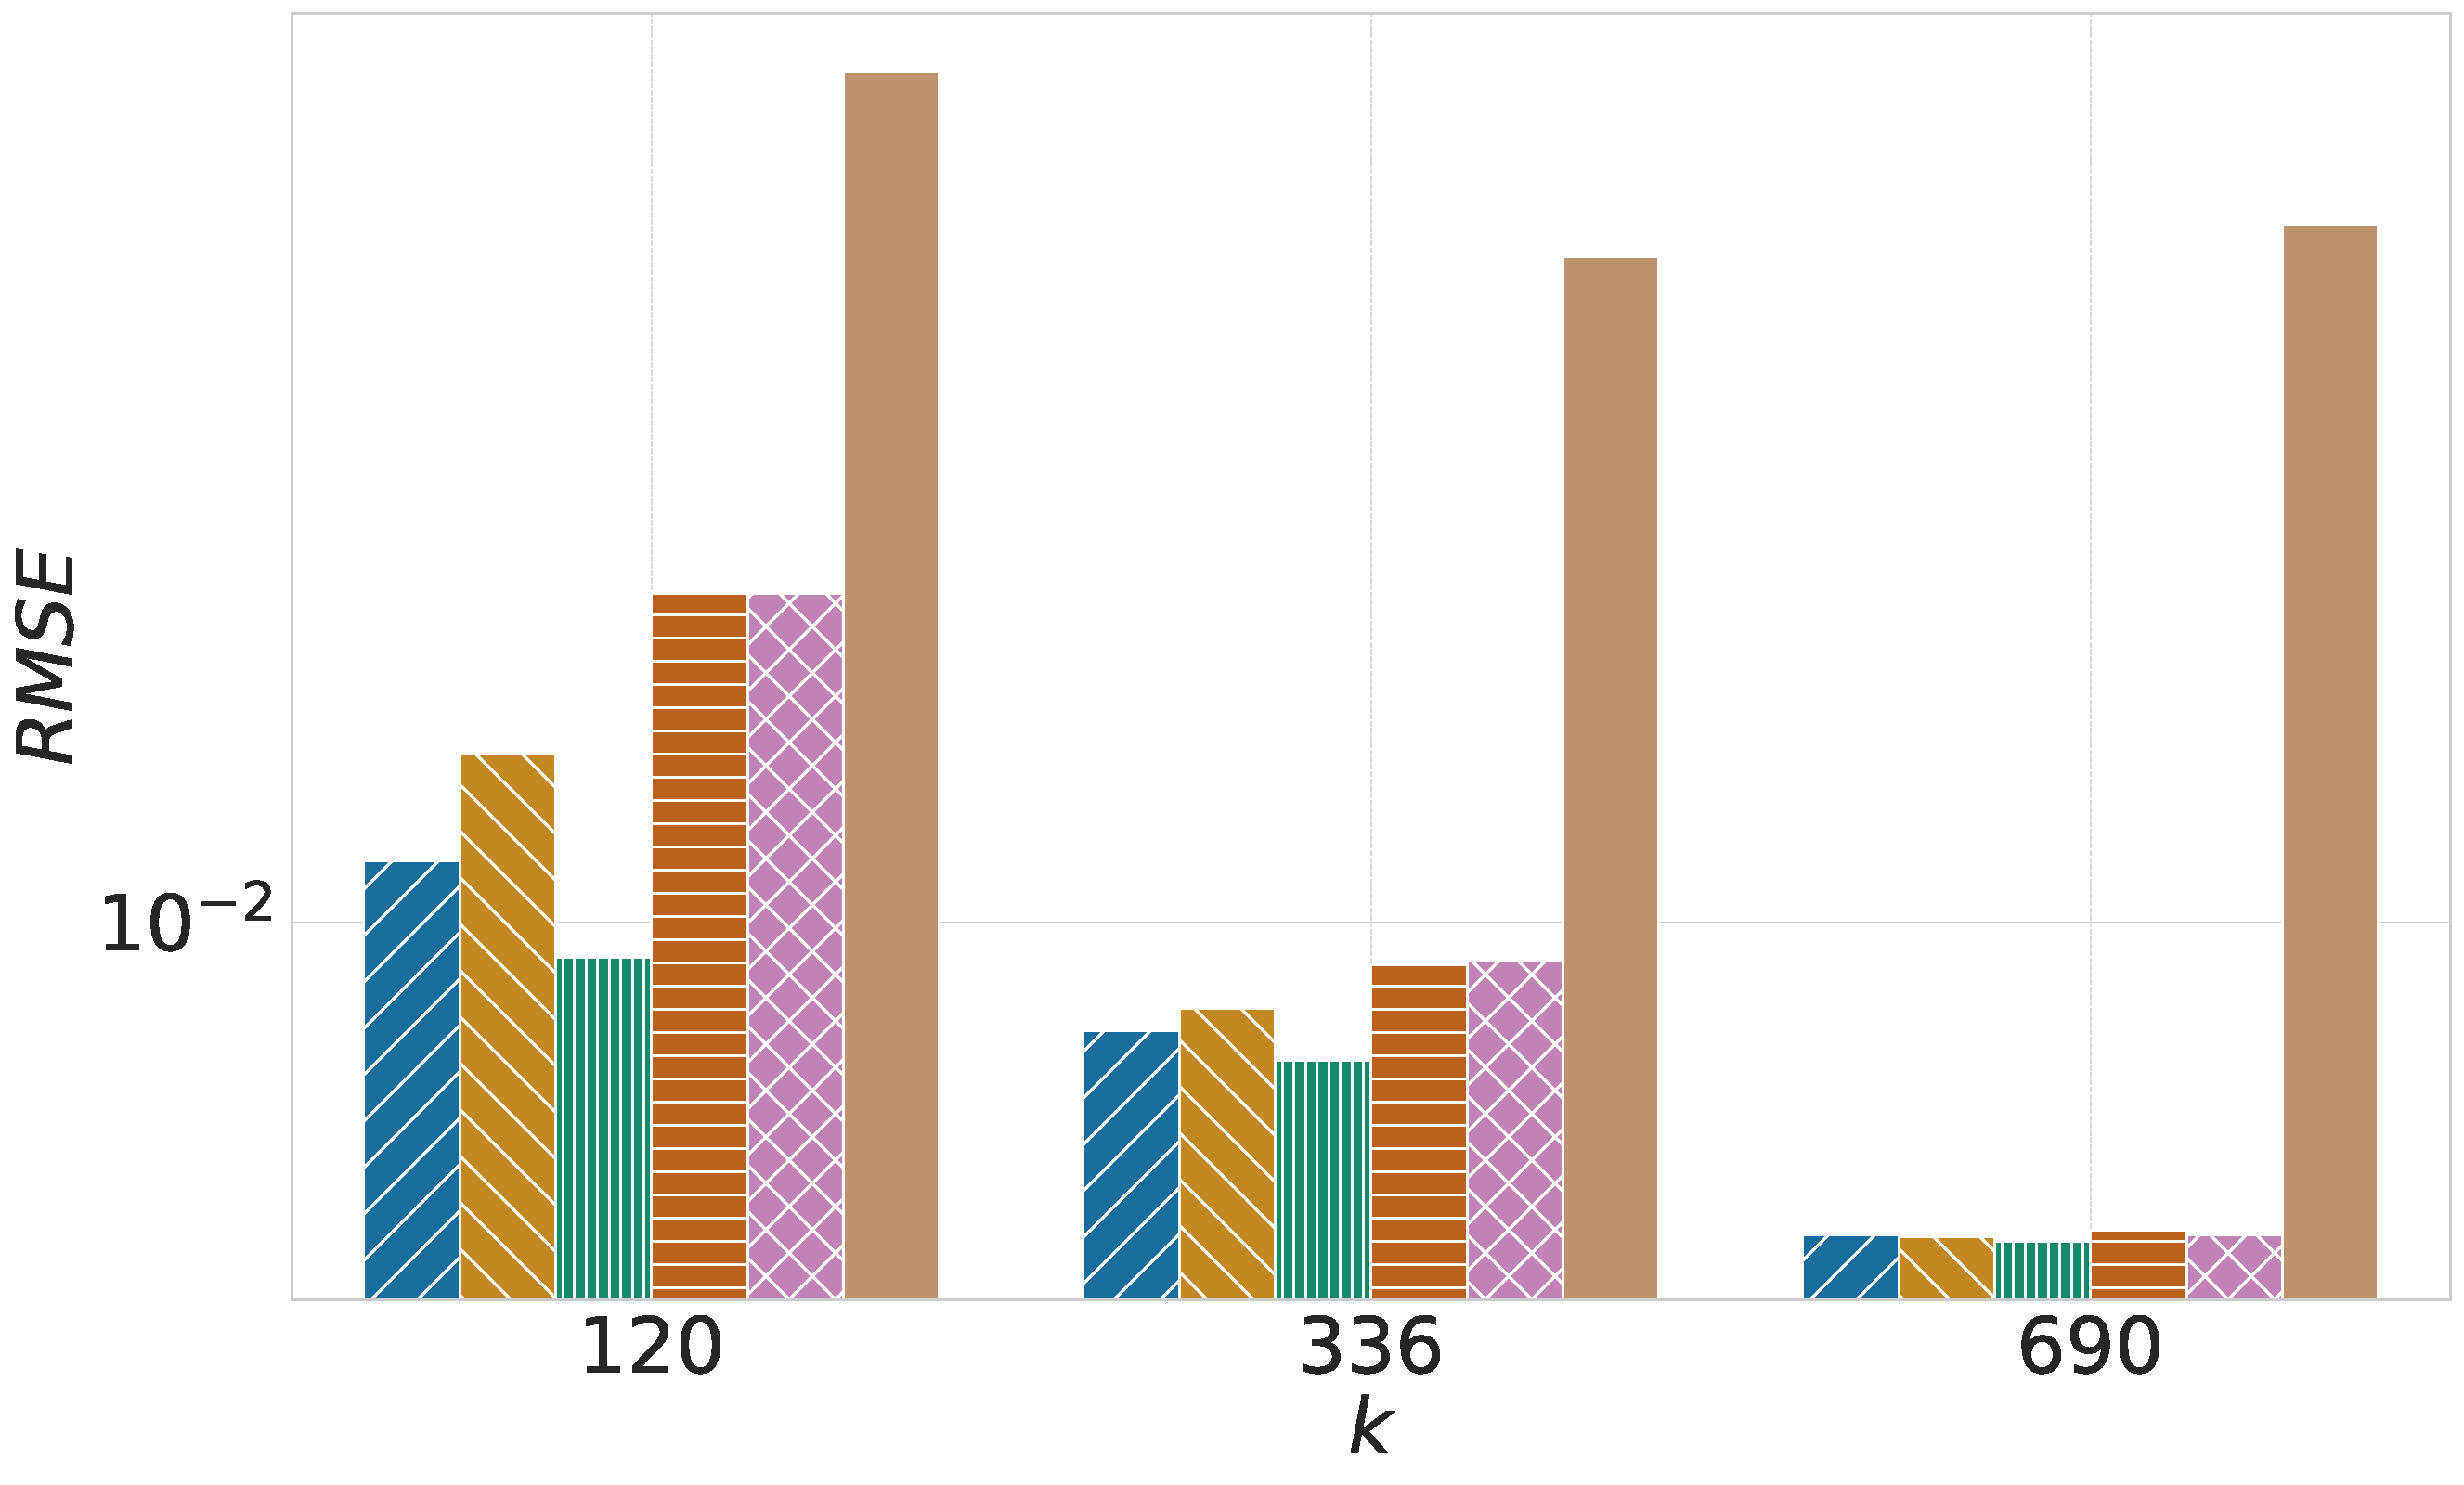
\includegraphics[width=\linewidth]{sections/figures/K_RMSE_BAR/rmse_compare_0.3_grid_avg_barchart_geo.pdf}
            \caption{Geolife with $\epsilon_{\infty}=0.3$}
            \label{fig:granularity_geo}
        \end{minipage}
        \hfill
        \begin{minipage}{0.8\textwidth}
            \centering
            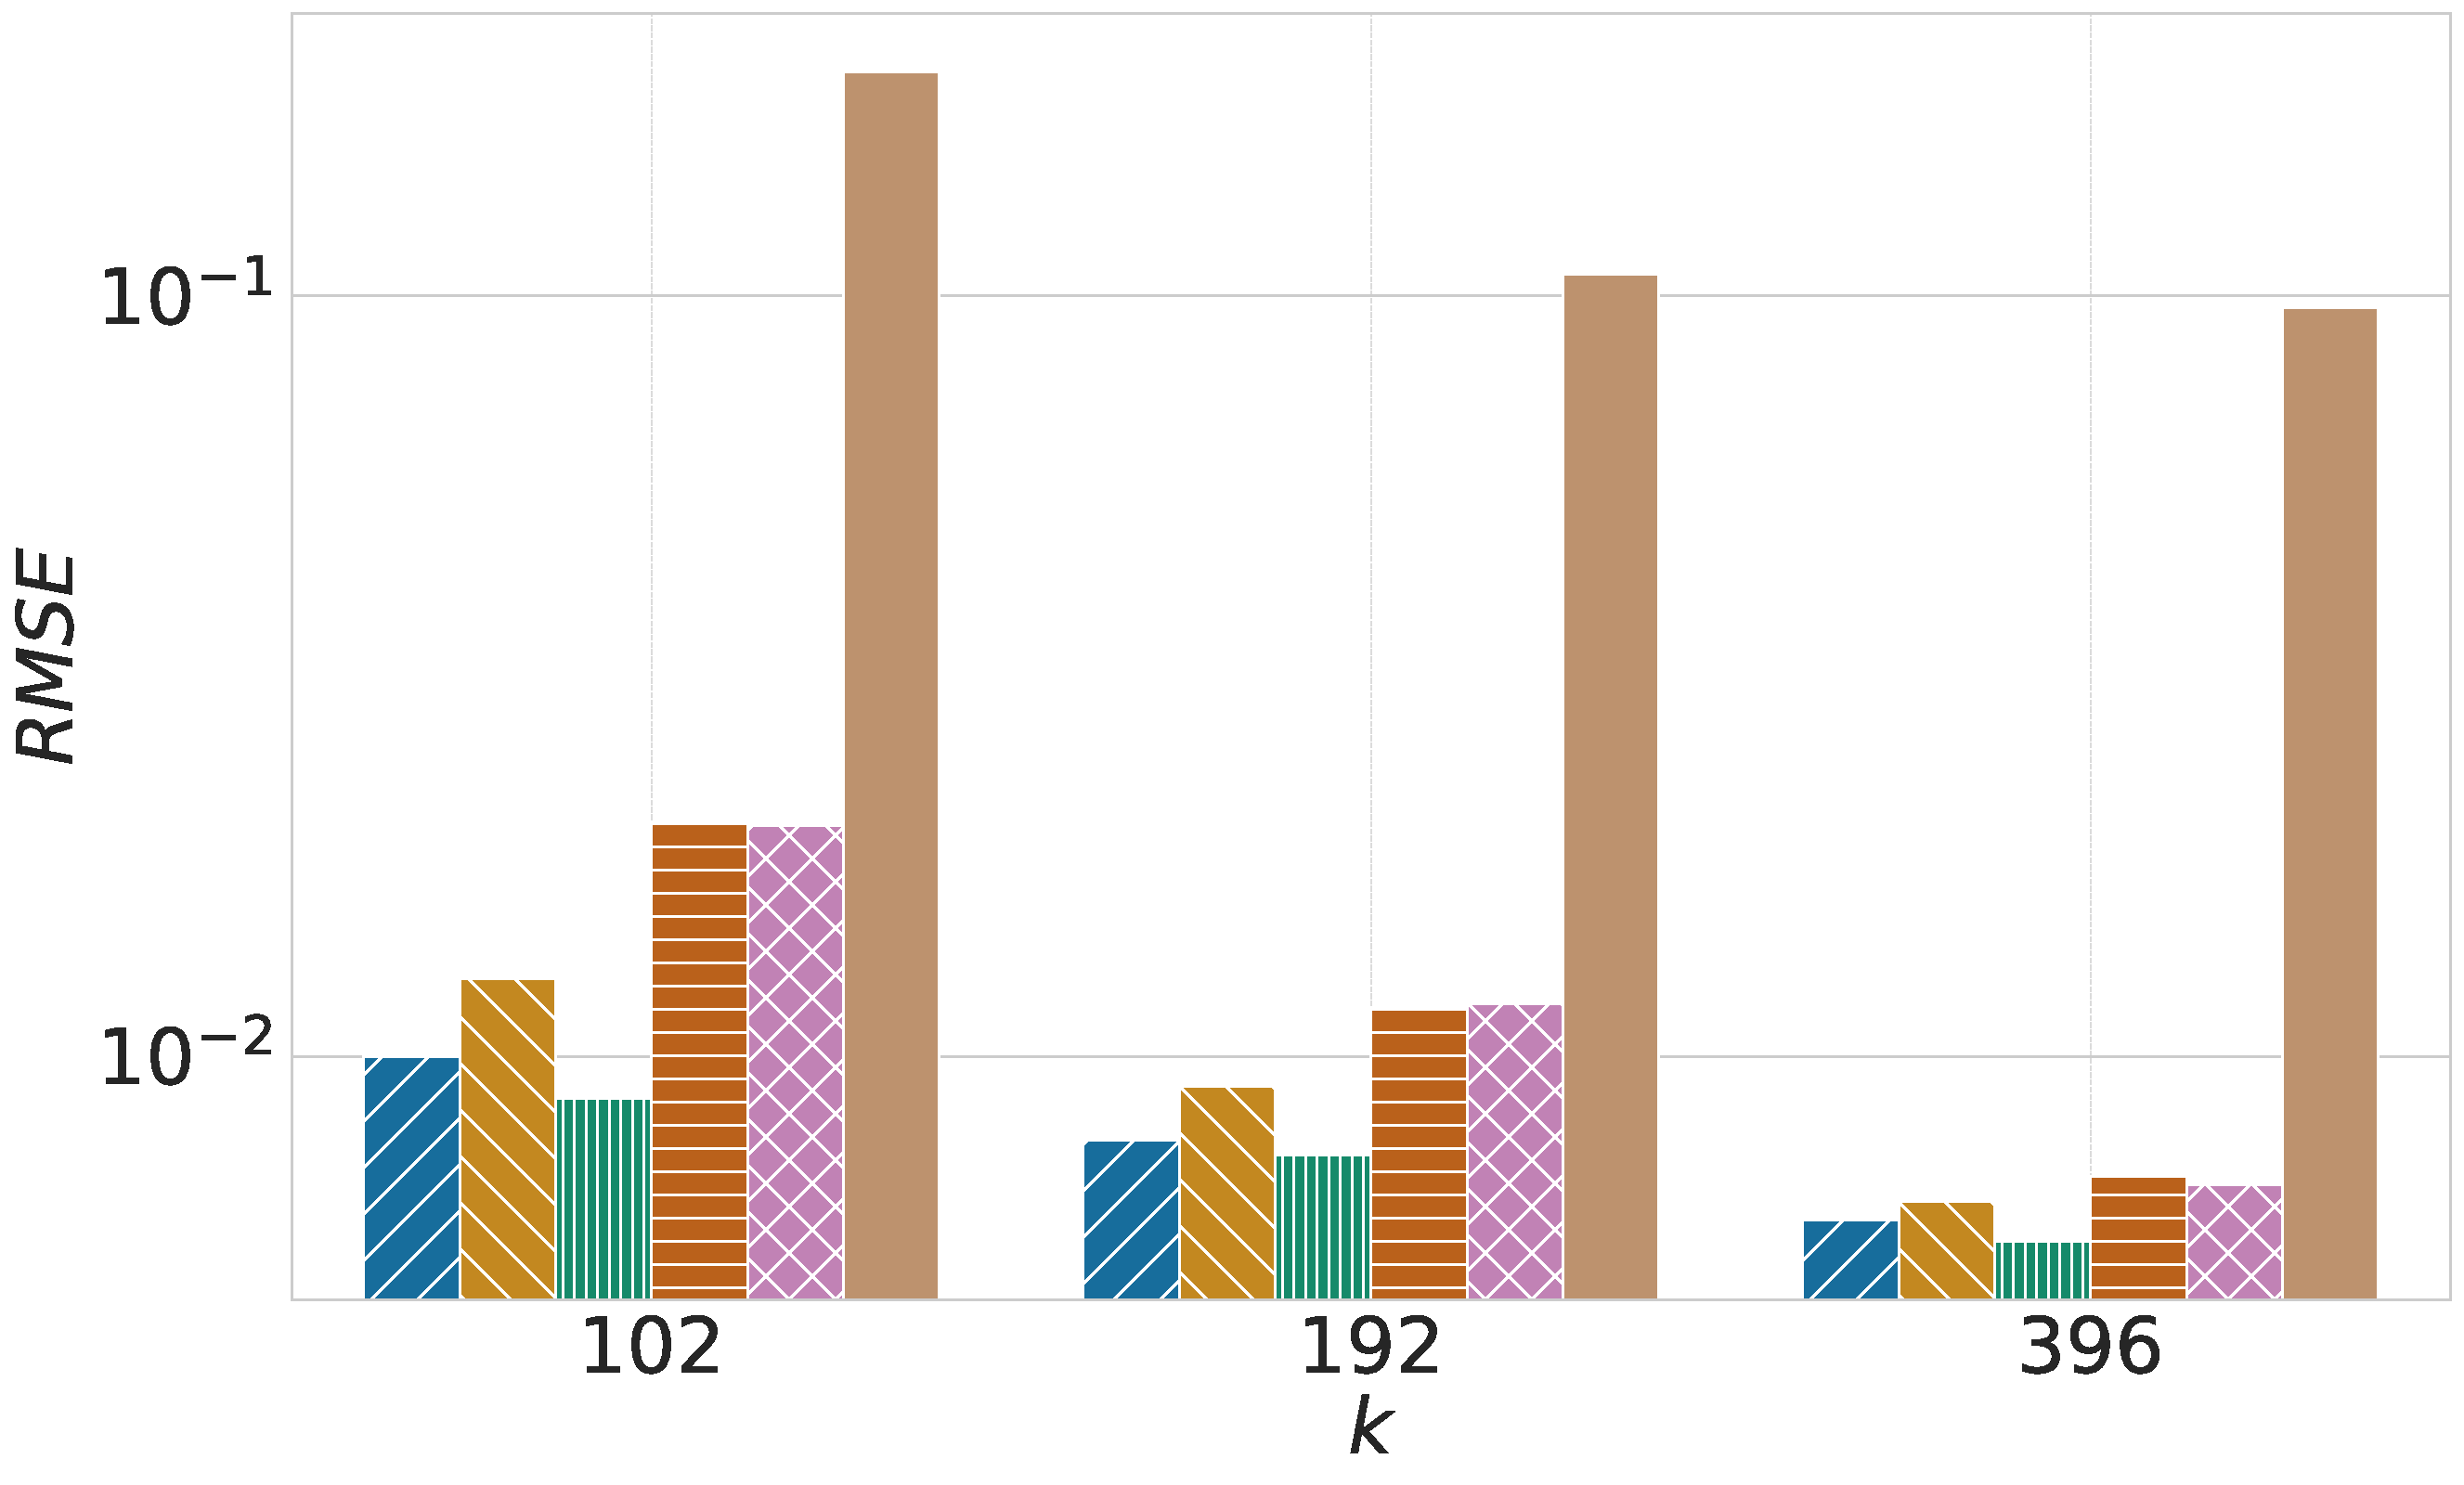
\includegraphics[width=\linewidth]{sections/figures/K_RMSE_BAR/rmse_compare_0.3_grid_avg_barchart_porto.pdf}
            \caption{Porto with $\epsilon_{\infty}=0.3$}
            \label{fig:granularity_porto}
        \end{minipage}
        \label{fig:sequence2}
    \end{subfigure}
    \caption{RMSE variation as a function of grid size for the four datasets: S1, S2, GeoLife, and Porto. Each chart represents the
error in data analysis when the initial grid size is set.}
\label{fig:granularity_barchart}
\end{figure}
Theoretically, the expected utility of each ALOG variant is influenced by the trade-off between noise magnitude (from LDP perturbation) and the granularity of the grid. According to the variance of LDP frequency estimation protocols such as LOSUE, the estimation variance is inversely proportional to the number of reports per grid cell. Thus uniform grid approaches (e.g., RAPPOR) are expected to exhibit higher error in regions with skewed data distributions due to non-uniformity error.

Figure \ref{fig:granularity_barchart} illustrates the effectiveness of our proposed adaptive grid approaches in enhancing utility compared to uniform grid-based methods, which consistently yielded the highest $RMSE$ across all scenarios. On the x-axis of the figure, $k$ represents the number of cells in the grid, while the y-axis shows the $RMSE$ between the real and estimated frequencies. Among the adaptive grid strategies, ALOG-2R emerged as the most effective, achieving the lowest $RMSE$ due to its two-round mechanism. In contrast, the ALOG-1R-b method demonstrated the poorest performance among the ALOG approaches. This is attributed to its reliance on a fixed base grid size during the grid adaptation process, which results in the loss of previously acquired knowledge and compromises its utility. For this experiment, a permanent privacy budget of 0.1 was used for each timestamp, and the adaptation window was set to 4.

\paragraph{Privacy Budget x Utility:}analyzing the relationship between the privacy budget and utility is crucial, as it highlights the trade-off between privacy guarantees and the accuracy of data estimates. A well-calibrated privacy budget establishes a balance, minimizing the $RMSE$ while ensuring adequate privacy protection. This balance is essential for practical deployments in applications involving sensitive data. \looseness=-1

In our experiments, we varied the privacy budget values between 0 and 1, with the budget representing the upper bound of privacy for each individual. We set up a cell size of $700 \, \text{meters} \times 700 \, \text{meters} $, which results in an initial grid granularity of $k = 225$ for datasets S1 and S2, $k = 336$ for Geolife, and $k = 192$ for Porto. The grid adaptation window was set to $w = 4$ moments of time. This setup allows us to explore how different privacy levels affect the utility of the system while maintaining the required privacy guarantees, as shown in Table \ref{tab:mse_budge}.


In the S1 and S2 datasets, ALOG-2R consistently achieves the lowest $RMSE$ values for all privacy budgets. This demonstrates how the two-stage model effectively enhances utility while maintaining compliance with privacy requirements. ALOG-1R-a follows closely, with slightly higher $RMSE$ values than ALOG-2R but significantly outperforming ALOG-1R-b.

The LOLOHA and LOSUE methods, while maintaining relatively stable performance across datasets, generally exhibit higher $RMSE$ values compared to ALOG-2R. Notably, RAPPOR, despite being a widely used method for privacy preservation, demonstrates the highest $RMSE$ values, particularly in scenarios with small privacy budgets, indicating its limitations in achieving high utility.

For the Geolife and Porto datasets, a similar pattern emerges. ALOG-2R continues to outperform other methods, achieving the best balance between privacy and utility. In the Geolife dataset, the $RMSE$ for ALOG-2R is consistently the lowest, especially for $\epsilon = 0.05$ and $\epsilon = 0.5$. In the Porto dataset, ALOG-2R again achieves the best results, with noticeable improvements over LOLOHA and LOSUE.  \looseness=-1 %This consistency across diverse datasets highlights the robustness of ALOG-2R as an adaptive grid method.

In summary, Table \ref{tab:mse_budge} emphasizes the significance of selecting an appropriate privacy budget $\epsilon$ and algorithm based on the application requirements. The results underscore the effectiveness of ALOG-2R in achieving a superior trade-off between privacy and utility, making it a strong candidate for practical deployments in sensitive data applications.

% \begin{table}[!tb]
% \centering
% \scriptsize
% \caption{RMSE ($\times 10^{-3}$) for $k=225$ in S1 and S2, $k=336$ in Geolife, and $k=192$ in Porto, with ALOG using $w=4$.}
% \begin{tabular}{c|c|cccccc}
% \toprule
% \textbf{DataSet} & \textbf{Budget}  & \textbf{ALOG-1R-a} & \textbf{ALOG-1R-b} & \textbf{ALOG-2R} & \textbf{LOLOHA} & \textbf{LOSUE} & \textbf{RAPPOR} \\
% \midrule
% \multirow{4}{*}{\textbf{S1}} 
% & $\epsilon = 0.05$ & 4.009 & 5.497 & \cellcolor{black!8}$\mathbf{3.908}$  & 6.948  & 6.924  & 1599.661  \\
% & $\epsilon = 0.1$  & 3.919  & 5.473  & \cellcolor{black!8}$\mathbf{3.866}$  & 7.124  & 6.960  & 1068.873  \\
% & $\epsilon = 0.5$  & 4.125  & 5.417  & \cellcolor{black!8}$\mathbf{3.771}$  & 6.882  & 6.884  & 153.428  \\
% & $\epsilon = 1.0$  & 3.998  & 5.406  & \cellcolor{black!8}$\mathbf{3.554}$  & 6.903  & 6.866  & 67.914  \\

% \midrule
% \multirow{3}{*}{\textbf{S2}} 
% & $\epsilon = 0.05$ & 4.314  & 5.953  & \cellcolor{black!8}$\mathbf{4.282}$  & 7.391  & 7.506  & 834.638  \\
% & $\epsilon = 0.1$  & 4.476  & 5.967  & \cellcolor{black!8}$\mathbf{4.212}$  & 7.516  & 7.536  & 666.694  \\
% & $\epsilon = 0.5$  & 4.389  & 6.009  & \cellcolor{black!8}$\mathbf{4.012}$  & 7.522  & 7.488  & 87.250  \\
% & $\epsilon = 1.0$  & 4.335  & 5.903  & \cellcolor{black!8}$\mathbf{4.102}$  & 7.749  & 7.489  & 112.595  \\
% \midrule

% \multirow{3}{*}{\textbf{Geolife}} 
% & $\epsilon = 0.05$ & 7.672  & 8.183  & \cellcolor{black!8}$\mathbf{6.694}$  & 9.053  & 9.162  & 432.922  \\
% & $\epsilon = 0.1$  & \cellcolor{black!8}$\mathbf{7.220}$  & 8.151  & 7.513  & 9.042  & 9.028  & 285.988  \\
% & $\epsilon = 0.5$  & 7.403  & 8.116  & \cellcolor{black!8}$\mathbf{6.855}$  & 9.001  & 9.190  & 77.613  \\
% & $\epsilon = 1.0$  & \cellcolor{black!8}$\mathbf{6.933}$  & 8.154  & 7.044  & 8.937  & 8.996  & 41.224  \\

% \midrule
% \multirow{3}{*}{\textbf{Porto}}
% & $\epsilon = 0.05$ & 7.522  & 9.211  & \cellcolor{black!8}$\mathbf{7.303}$  & 11.358  & 11.320  & 829.024  \\
% & $\epsilon = 0.1$  & 7.657  & 8.720  & \cellcolor{black!8}$\mathbf{7.151}$  & 11.524  & 11.831  & 197.978  \\
% & $\epsilon = 0.5$  & 7.831  & 8.796  & \cellcolor{black!8}$\mathbf{6.886}$  & 11.778  & 11.332  & 111.164  \\
% & $\epsilon = 1.0$  & 7.474  & 8.907  & \cellcolor{black!8}$\mathbf{6.876}$  & 11.704  & 11.444  & 68.865  \\

% \bottomrule
% \end{tabular}
% \label{tab:mse_budge}
% \end{table}

% \newcolumntype{L}{>{\raggedright\arraybackslash}X} % Left-aligned X column
% \newcolumntype{C}{>{\centering\arraybackslash}X}   % Centered X column
% \newcolumntype{R}{>{\raggedleft\arraybackslash}X}  % Right-aligned X column

\begin{table*}
\centering
% \small
\caption{RMSE ($\times 10^{-3}$) for $k=225$ in S1 and S2, $k=336$ in Geolife, and $k=192$ in Porto, with ALOG using $w=4$.}
\begin{tabular}{c|c|cccccc}
\toprule
\textbf{DataSet} & \textbf{Budget}  & \textbf{ALOG-1R-a} & \textbf{ALOG-1R-b} & \textbf{ALOG-2R} & \textbf{LOLOHA} & \textbf{LOSUE} & \textbf{RAPPOR} \\
\midrule
\multirow{4}{*}{\textbf{S1}} 
& $\epsilon = 0.05$ & 4.009 & 5.497 & \cellcolor{black!8}$\mathbf{3.908}$  & 6.948  & 6.924  & 1599.661  \\
& $\epsilon = 0.1$  & 3.919  & 5.473  & \cellcolor{black!8}$\mathbf{3.866}$  & 7.124  & 6.960  & 1068.873  \\
& $\epsilon = 0.5$  & 4.125  & 5.417  & \cellcolor{black!8}$\mathbf{3.771}$  & 6.882  & 6.884  & 153.428  \\
& $\epsilon = 1.0$  & 3.998  & 5.406  & \cellcolor{black!8}$\mathbf{3.554}$  & 6.903  & 6.866  & 67.914  \\

\midrule
\multirow{3}{*}{\textbf{S2}} 
& $\epsilon = 0.05$ & 4.314  & 5.953  & \cellcolor{black!8}$\mathbf{4.282}$  & 7.391  & 7.506  & 834.638  \\
& $\epsilon = 0.1$  & 4.476  & 5.967  & \cellcolor{black!8}$\mathbf{4.212}$  & 7.516  & 7.536  & 666.694  \\
& $\epsilon = 0.5$  & 4.389  & 6.009  & \cellcolor{black!8}$\mathbf{4.012}$  & 7.522  & 7.488  & 87.250  \\
& $\epsilon = 1.0$  & 4.335  & 5.903  & \cellcolor{black!8}$\mathbf{4.102}$  & 7.749  & 7.489  & 112.595  \\
\midrule

\multirow{3}{*}{\textbf{Geolife}} 
& $\epsilon = 0.05$ & 7.672  & 8.183  & \cellcolor{black!8}$\mathbf{6.694}$  & 9.053  & 9.162  & 432.922  \\
& $\epsilon = 0.1$  & \cellcolor{black!8}$\mathbf{7.220}$  & 8.151  & 7.513  & 9.042  & 9.028  & 285.988  \\
& $\epsilon = 0.5$  & 7.403  & 8.116  & \cellcolor{black!8}$\mathbf{6.855}$  & 9.001  & 9.190  & 77.613  \\
& $\epsilon = 1.0$  & \cellcolor{black!8}$\mathbf{6.933}$  & 8.154  & 7.044  & 8.937  & 8.996  & 41.224  \\

\midrule
\multirow{3}{*}{\textbf{Porto}}
& $\epsilon = 0.05$ & 7.522  & 9.211  & \cellcolor{black!8}$\mathbf{7.303}$  & 11.358  & 11.320  & 829.024  \\
& $\epsilon = 0.1$  & 7.657  & 8.720  & \cellcolor{black!8}$\mathbf{7.151}$  & 11.524  & 11.831  & 197.978  \\
& $\epsilon = 0.5$  & 7.831  & 8.796  & \cellcolor{black!8}$\mathbf{6.886}$  & 11.778  & 11.332  & 111.164  \\
& $\epsilon = 1.0$  & 7.474  & 8.907  & \cellcolor{black!8}$\mathbf{6.876}$  & 11.704  & 11.444  & 68.865  \\

\bottomrule
\end{tabular}
\label{tab:mse_budge}
\end{table*}

\paragraph{Longitudinal Setting x Utility:}another important aspect to consider is the impact of data's longitudinal nature on utility. Figure \ref{fig:longitudinality_barchart} illustrates how the temporal evolution of data affects the performance of privacy-preserving mechanisms, which is crucial for applications that involve dynamic and continuously changing datasets. Understanding this impact allows us to assess the robustness of adaptive grid methods, such as ALOG-2R, in maintaining low $RMSE$ while addressing the challenges posed by temporal variations in data distribution. This analysis will further provide insights into how privacy budgets and grid adaptations interact over time, ensuring the methods remain effective in real-world scenarios with longitudinal data.

Figure \ref{fig:longitudinality_barchart} consists of four subcharts, each corresponding to a different data set. These graphs illustrate the relationship between the number of consecutive reports sent by users and the $RMSE$. In the preceding analysis, RAPPOR consistently demonstrated significantly poorer performance compared to the other methods (as seen in Figure \ref{fig:granularity_barchart} and Table \ref{tab:mse_budge}). To provide a clearer visualization and focus on the comparative differences among the higher-performing approaches, RAPPOR was excluded from Figure \ref{fig:longitudinality_barchart}. However, it is important to note that the trend of RAPPOR's inferior performance continues in this subsequent analysis, though not shown for visual clarity. \looseness=-1

The ALOG approaches exhibit much better performance, with ALOG-2R and ALOG-1R-a showing very similar results, often achieving the lowest $RMSE$ values. These methods leverage their adaptive mechanisms to outperform not only RAPPOR but also other approaches like LOSUE and LOLOHA, which perform moderately but fail to match the precision of ALOG methods.

The consistent superiority of ALOG-2R and ALOG-1R-a across datasets highlights their adaptability and efficiency, particularly in scenarios with a higher frequency of consecutive user requests. These results underline the importance of selecting advanced adaptive grid methods to ensure low $RMSE$ in privacy-preserving systems.
% 
\begin{figure*}[!tb]
    \centering
    \Description{longitudinality plots}
    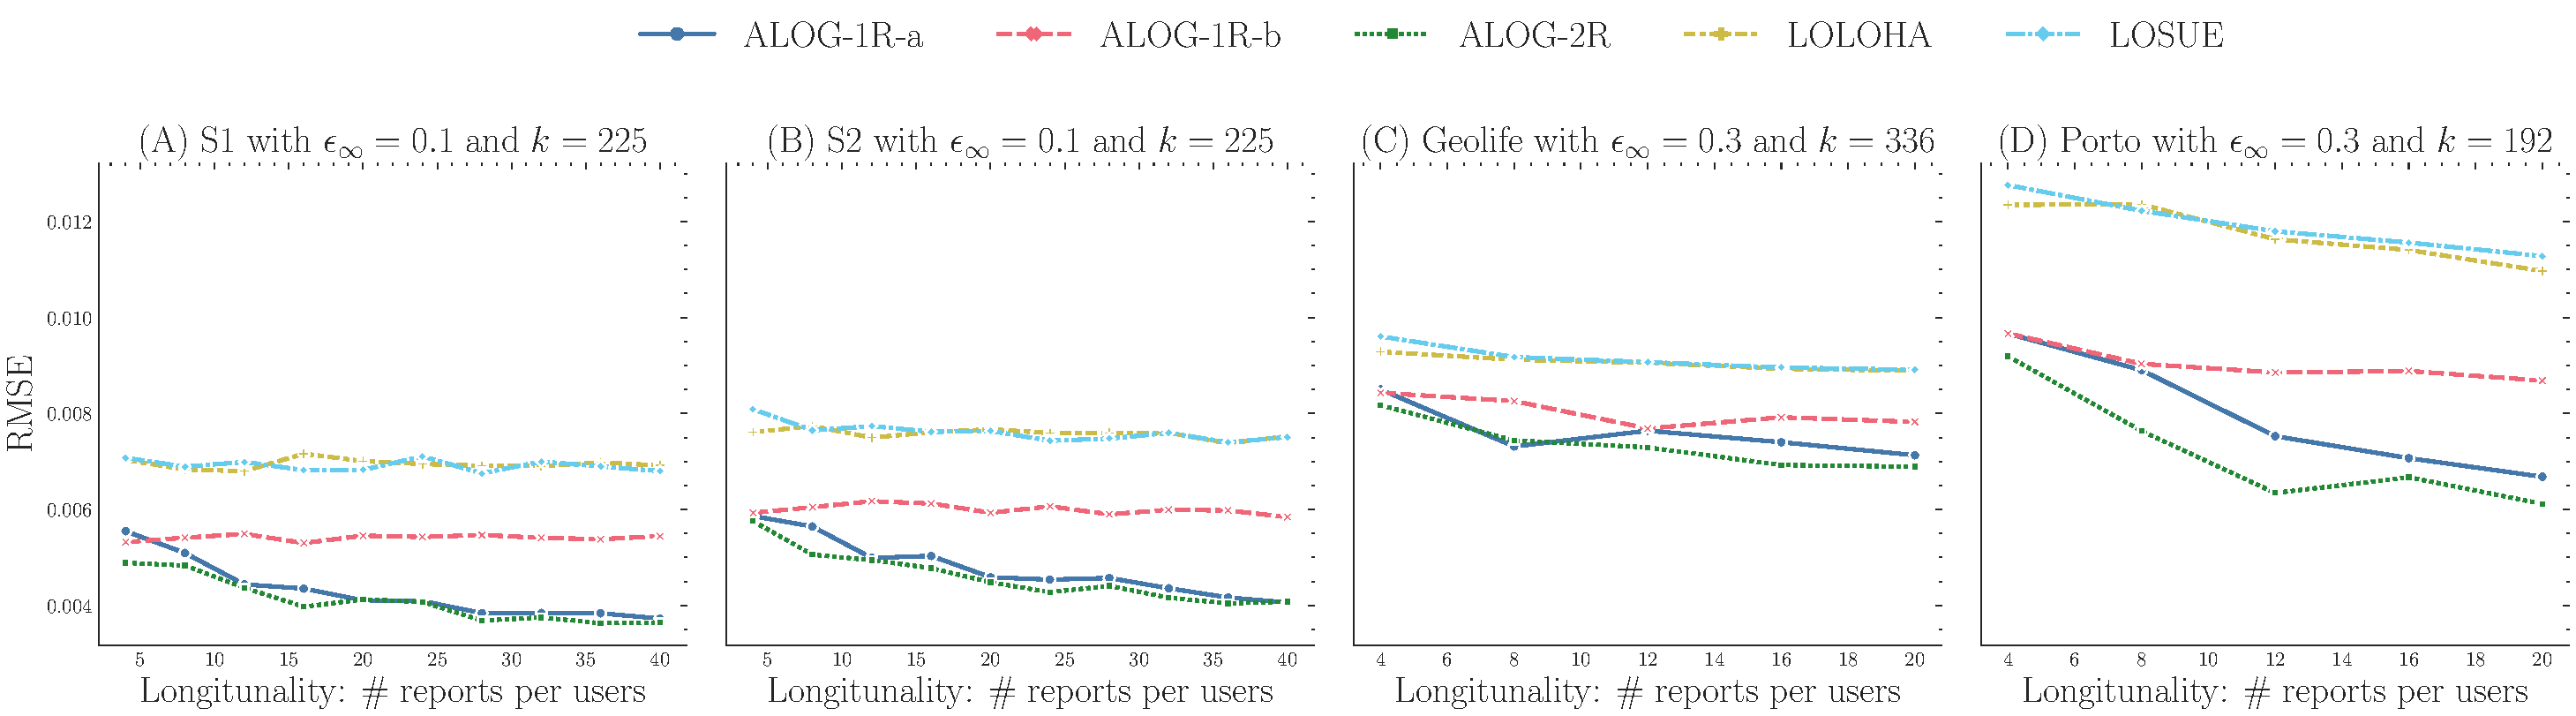
\includegraphics[width=\linewidth]{sections/figures/res_num_points.pdf}
    \caption{RMSE variation with the number of reports per user for the four datasets: S1, S2, GeoLife, and Porto.}
    \label{fig:longitudinality_barchart}
\end{figure*}

\paragraph{Budget Consumption:}we now begin a new analysis focusing on the budget privacy consumption. As shown in Table \ref{fig:bC_MSE}, the ALOG approaches demonstrate the highest budget consumption among the methods. This is expected since the grid adaptation process inherent to ALOG methods sacrifices a key efficiency mechanism available in other approaches: memoization. Memoization enables non-adaptive methods like LOLOHA, LOSUE, and RAPPOR to conserve the privacy budget by reusing previously computed information.

Despite this drawback, we now extend our analysis to explicitly evaluate privacy budget consumption using Pareto frontier analysis (Figure \ref{fig:res_pareto}). The Pareto frontiers reveal a clear efficiency-accuracy trade-off among the evaluated methods. Methods located closer to the frontier indicate superior performance, characterized by achieving lower RMSE at minimal budget consumption.

In the synthetic datasets, LOLOHA remains close to the frontier only under conditions of very low privacy budget consumption. In contrast, adaptive methods such as ALOG-2R and ALOG-1R-a dominate all other approaches at higher budget levels, consistently achieving lower RMSE values. For the GeoLife dataset, ALOG-2R and ALOG-1R-a outperform other methods starting from privacy budget consumptions above approximately $0.35$ and $0.29$, respectively. Similarly, for the Porto dataset, ALOG-1R-a dominates at budget consumptions exceeding $0.9$, whereas ALOG-2R surpasses all other methods once the budget exceeds $1.0$.

Non-adaptive methods, including LOLOHA, LOSUE, and RAPPOR, consistently demonstrate lower budget consumption due to memoization; however, their positions farther from the Pareto frontier clearly illustrate their limitations in accuracy compared to adaptive grid-based approaches.

\begin{figure*}[!tb]
    \centering
    \Description{budget paretto}
    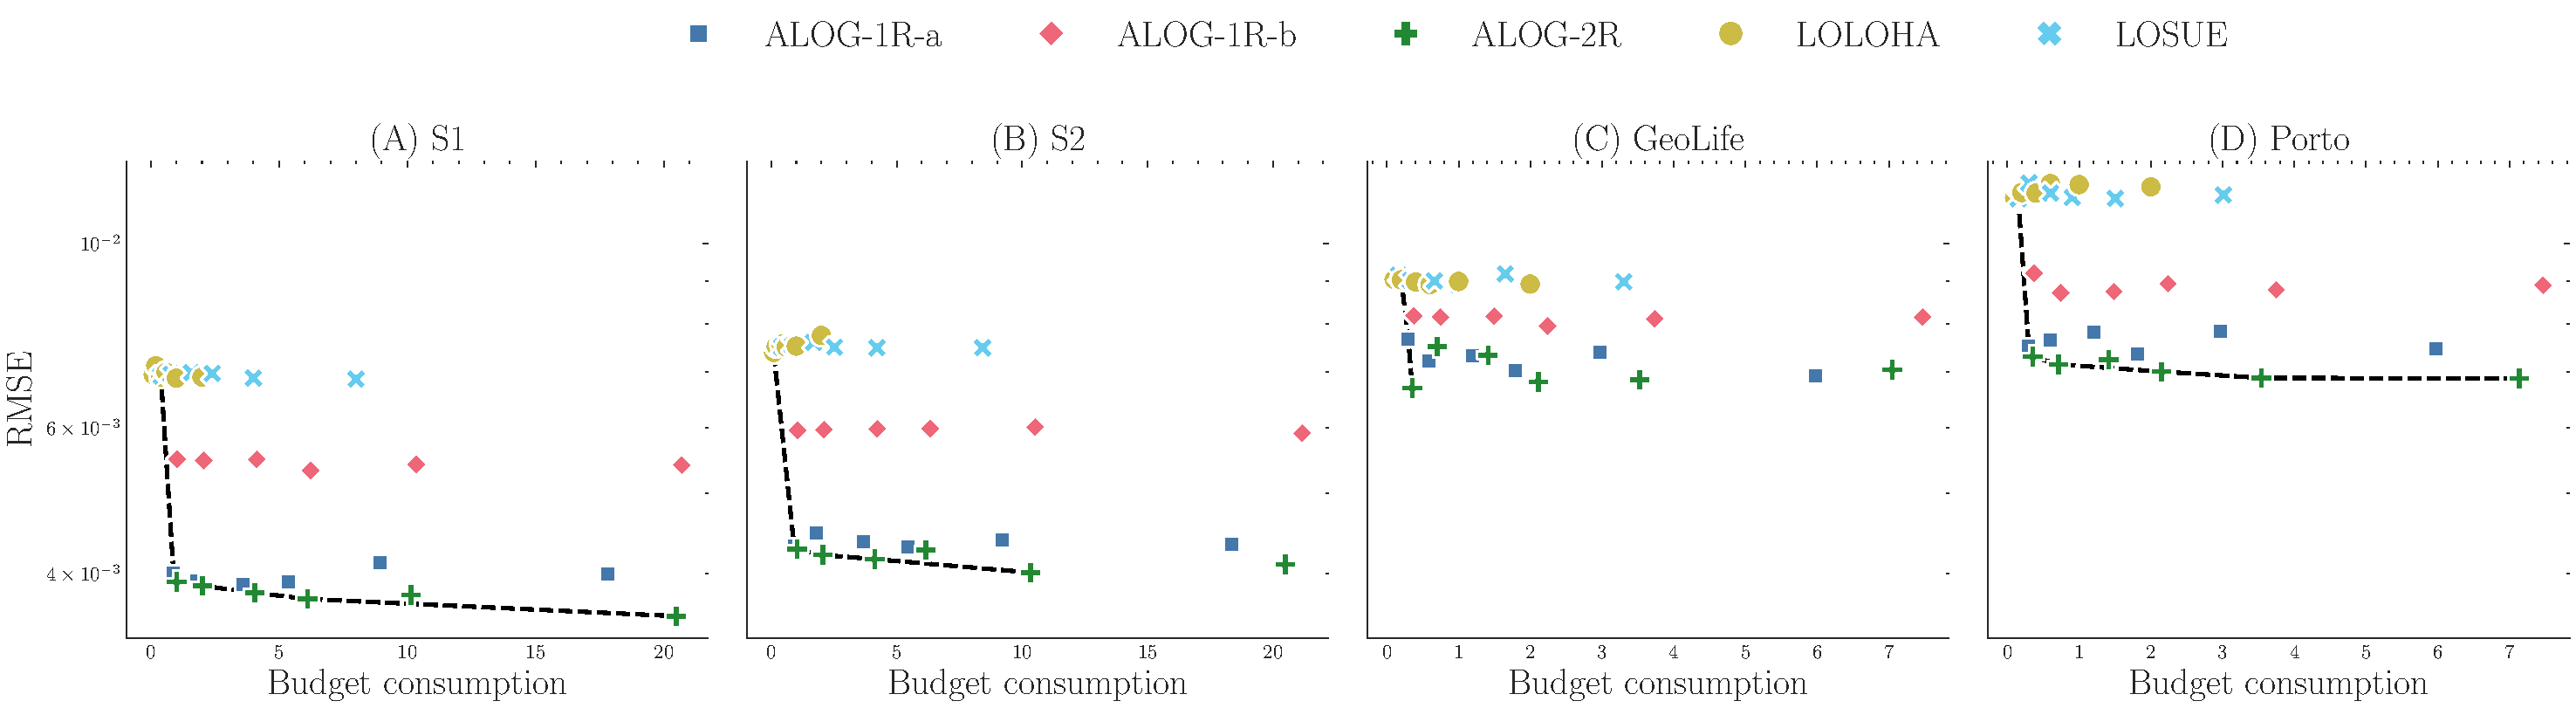
\includegraphics[width=\linewidth]{sections/figures/res_pareto.pdf}
    \caption{The Pareto frontier (black dashed line) demonstrates ALOG's superior trade-off between error (RMSE) and privacy budget consumption. Our method dominates the frontier in nearly all operational scenarios, establishing it as the preferred choice for most practical applications. Only in a narrow range of extremely low budget conditions does LOLOHA show marginally better performance.}
    \label{fig:res_pareto}
\end{figure*}

These results highlight that while ALOG approaches are more demanding in terms of budget consumption, their superior utility makes them highly advantageous for applications where accuracy and adaptability are critical, even in longitudinal settings.

% Non-adaptive methods, including LOLOHA, LOSUE, and RAPPOR, consistently demonstrate lower budget consumption due to memoization; however, their positions farther from the Pareto frontier clearly illustrate their limitations in accuracy compared to adaptive grid-based approaches. In contrast, while ALOG approaches are more demanding in terms of budget consumption, their superior utility, particularly in longitudinal settings, makes them highly advantageous for applications where accuracy and adaptability are critical.



% \begin{table*}[h!]
% \centering
% \small
% \caption{Budget Consumption for Datasets S1, S2, Geolife and Porto}
% \begin{tabular}{c|cccccc}
% \toprule
% \textbf{DataSet} & \textbf{ALOG-1R-a} & \textbf{ALOG-1R-b} & \textbf{ALOG-2R} & \textbf{LOLOHA} & \textbf{LOSUE} & \textbf{RAPPOR} \\
% \midrule
% S1 & \cellcolor{black!8}$\mathbf{1.78} $ & $2.07 $ & $2.02 $ & \cellcolor{black!8}$\mathbf{0.2}$ & $0.80$ & $0.80$ \\
% S2 & \cellcolor{black!8}$\mathbf{1.84} $ & $2.11 $ & $2.05 $ & \cellcolor{black!8}$\mathbf{0.2} $ & $0.84 $ & $0.86 $ \\
% Geolife & \cellcolor{black!8}$\mathbf{1.78} $ & $2.24 $ & $2.10 $ & \cellcolor{black!8}$\mathbf{0.59} $ & $0.99 $ & $0.99 $ \\
% Porto & \cellcolor{black!8}$\mathbf{1.78} $ & $2.07 $ & $2.02 $ & \cellcolor{black!8}$\mathbf{0.2}$ & $0.801$ & $0.801$ \\
% \bottomrule
% \end{tabular}
% \label{fig:bC_MSE}
% \end{table*}
% 
\begin{table}[!tb]
\centering
\footnotesize % or \footnotesize
\caption{Budget Consumption for Datasets S1, S2, Geolife and Porto}
\begin{tabular}{c|cccccc}
% \begin{tabularx}{\columnwidth}{@{}c|cccccc@{}}
% \begin{tabularx}{\columnwidth}{@{} L | C | C C C C C C @{}}
\toprule
\textbf{\makecell{DataSet}} & \textbf{\makecell{ALOG \\ 1R-a}} & \textbf{\makecell{ALOG \\ 1R-b}} & \textbf{\makecell{ALOG \\ 2R}} & \textbf{LOLOHA} & \textbf{LOSUE} & \textbf{RAPPOR} \\
\midrule
S1 & \cellcolor{black!8}$\mathbf{1.78} $ & $2.07 $ & $2.02 $ & \cellcolor{black!8}$\mathbf{0.2}$ & $0.80$ & $0.80$ \\
S2 & \cellcolor{black!8}$\mathbf{1.84} $ & $2.11 $ & $2.05 $ & \cellcolor{black!8}$\mathbf{0.2} $ & $0.84 $ & $0.86 $ \\
Geolife & \cellcolor{black!8}$\mathbf{1.78} $ & $2.24 $ & $2.10 $ & \cellcolor{black!8}$\mathbf{0.59} $ & $0.99 $ & $0.99 $ \\
Porto & \cellcolor{black!8}$\mathbf{1.78} $ & $2.07 $ & $2.02 $ & \cellcolor{black!8}$\mathbf{0.2}$ & $0.801$ & $0.801$ \\
\bottomrule
\end{tabular}
\label{fig:bC_MSE}
\end{table}
% 
\begin{figure*}[!ht]
    \centering
    \Description{window plots}
    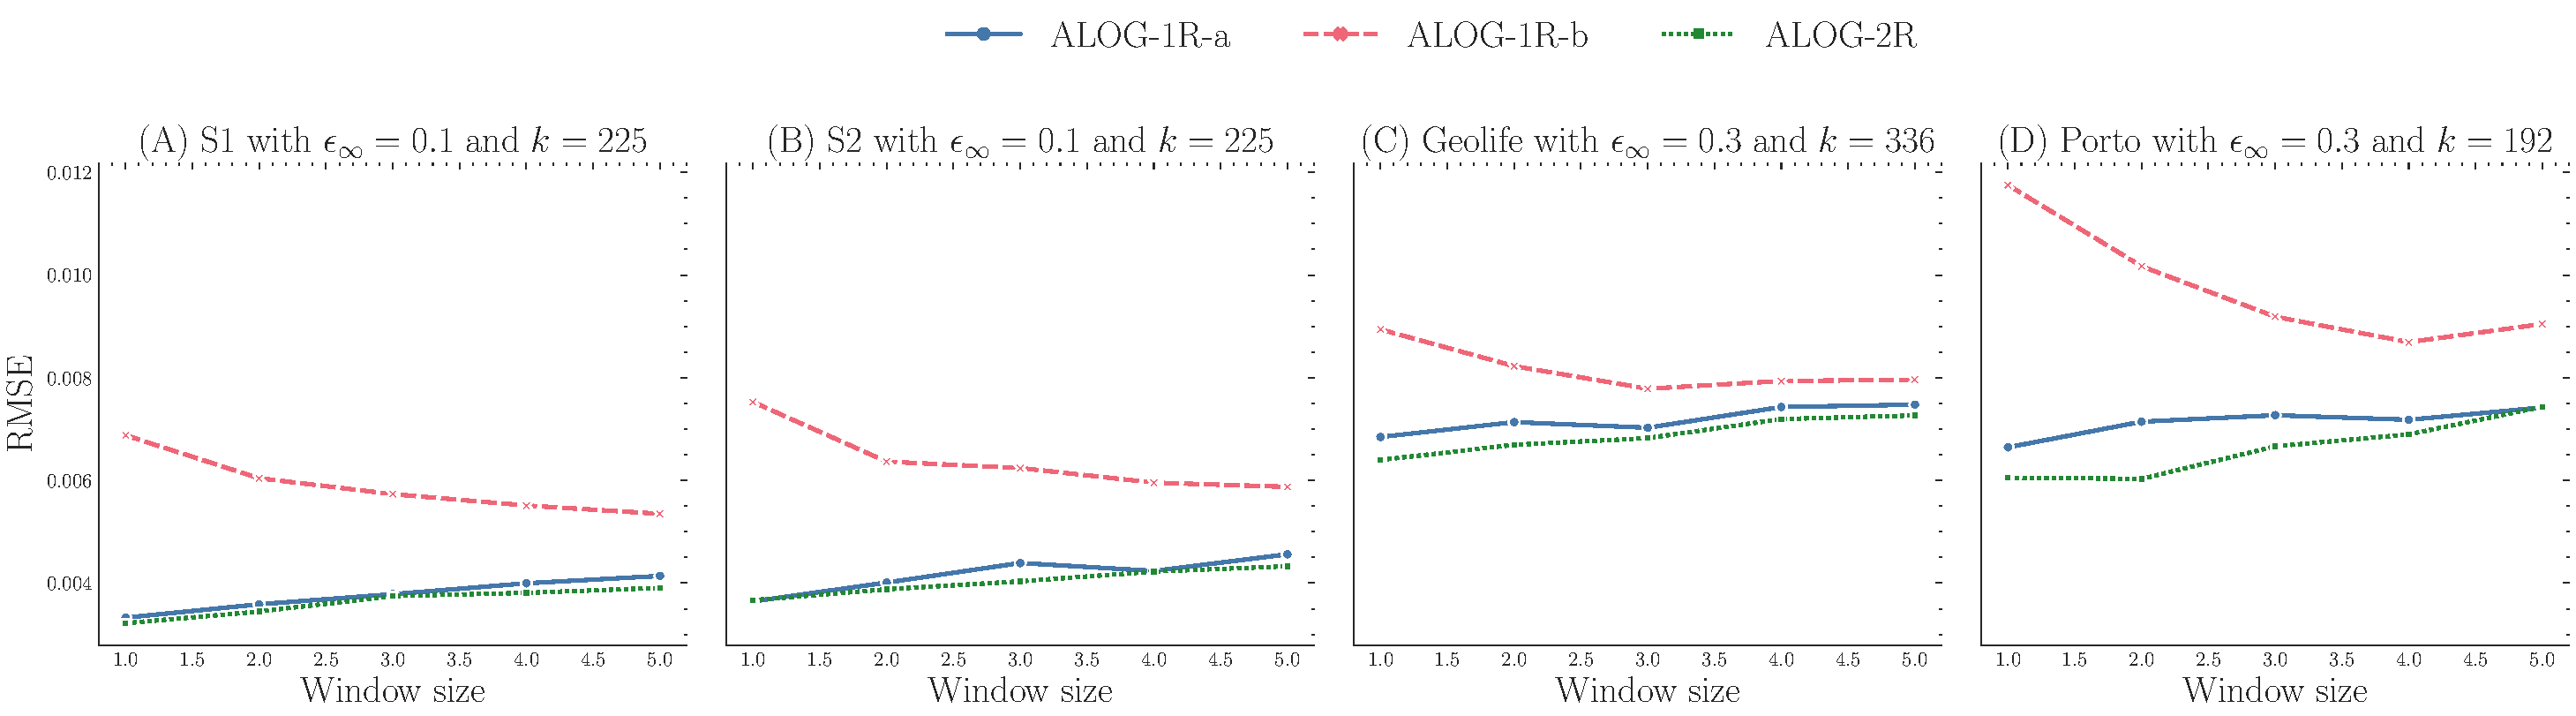
\includegraphics[width=\linewidth]{sections/figures/res_windows.pdf}
    \caption{RMSE variation in terms of the grid adaptation window size for the four datasets: S1, S2, GeoLife, and Porto.}
    \label{fig:Window_linechart}
\end{figure*}

\paragraph{GAW x Utility:}the grid adaptation window plays a crucial role in the performance of the ALOG approaches. Since all three ALOG variants consistently outperform uniform grid approaches, it is essential to understand their behavior in terms of grid size and how it affects their utility.

Figure \ref{fig:Window_linechart} illustrates that ALOG-2R and ALOG-1R-a maintain better utility across all tested window sizes for each dataset. However, a notable trend emerges: as the window size increases, the error for ALOG-2R and ALOG-1R-a also increases. Conversely, ALOG-1R-b demonstrates a decreasing error trend as the window size grows. This divergence arises from the distinct grid adaptation mechanisms employed by these approaches.

ALOG-1R-a and ALOG-2R experience an increase in error with larger window sizes primarily due to their reliance on the previous grid for adaptation. These methods dynamically split grid cells to increase granularity when needed but lack the ability to reduce granularity by merging cells as data density decreases. This limitation becomes more pronounced as the window size grows because larger windows lead to greater variations in data distribution over time. The inability to decrease granularity hinders their ability to adjust effectively to these abrupt changes, resulting in inefficiencies and increased error.

In contrast, ALOG-1R-b demonstrates better performance in scenarios with larger window sizes due to its use of a fixed base grid during the adaptation process. This design allows ALOG-1R-b to reset and adjust more effectively to significant changes in data distribution, making it more resilient to abrupt shifts that occur when the window size is larger. By avoiding reliance on a previous grid, ALOG-1R-b can maintain alignment with current data density, ensuring more consistent and efficient performance even under challenging conditions. This highlights the importance of adaptability in handling varying data dynamics, particularly in scenarios with large adaptation windows.

In summary, the increasing error trend for ALOG-2R and ALOG-1R-a with larger window sizes is a consequence of their grid adaptation process, which cannot shrink the grid when necessary. ALOG-1R-b, with its reliance on a base grid, provides better adjustment and resilience to data dynamics over longer periods, highlighting the trade-offs inherent in these adaptive strategies.


% \begin{figure*}[!ht]
%     \centering
%     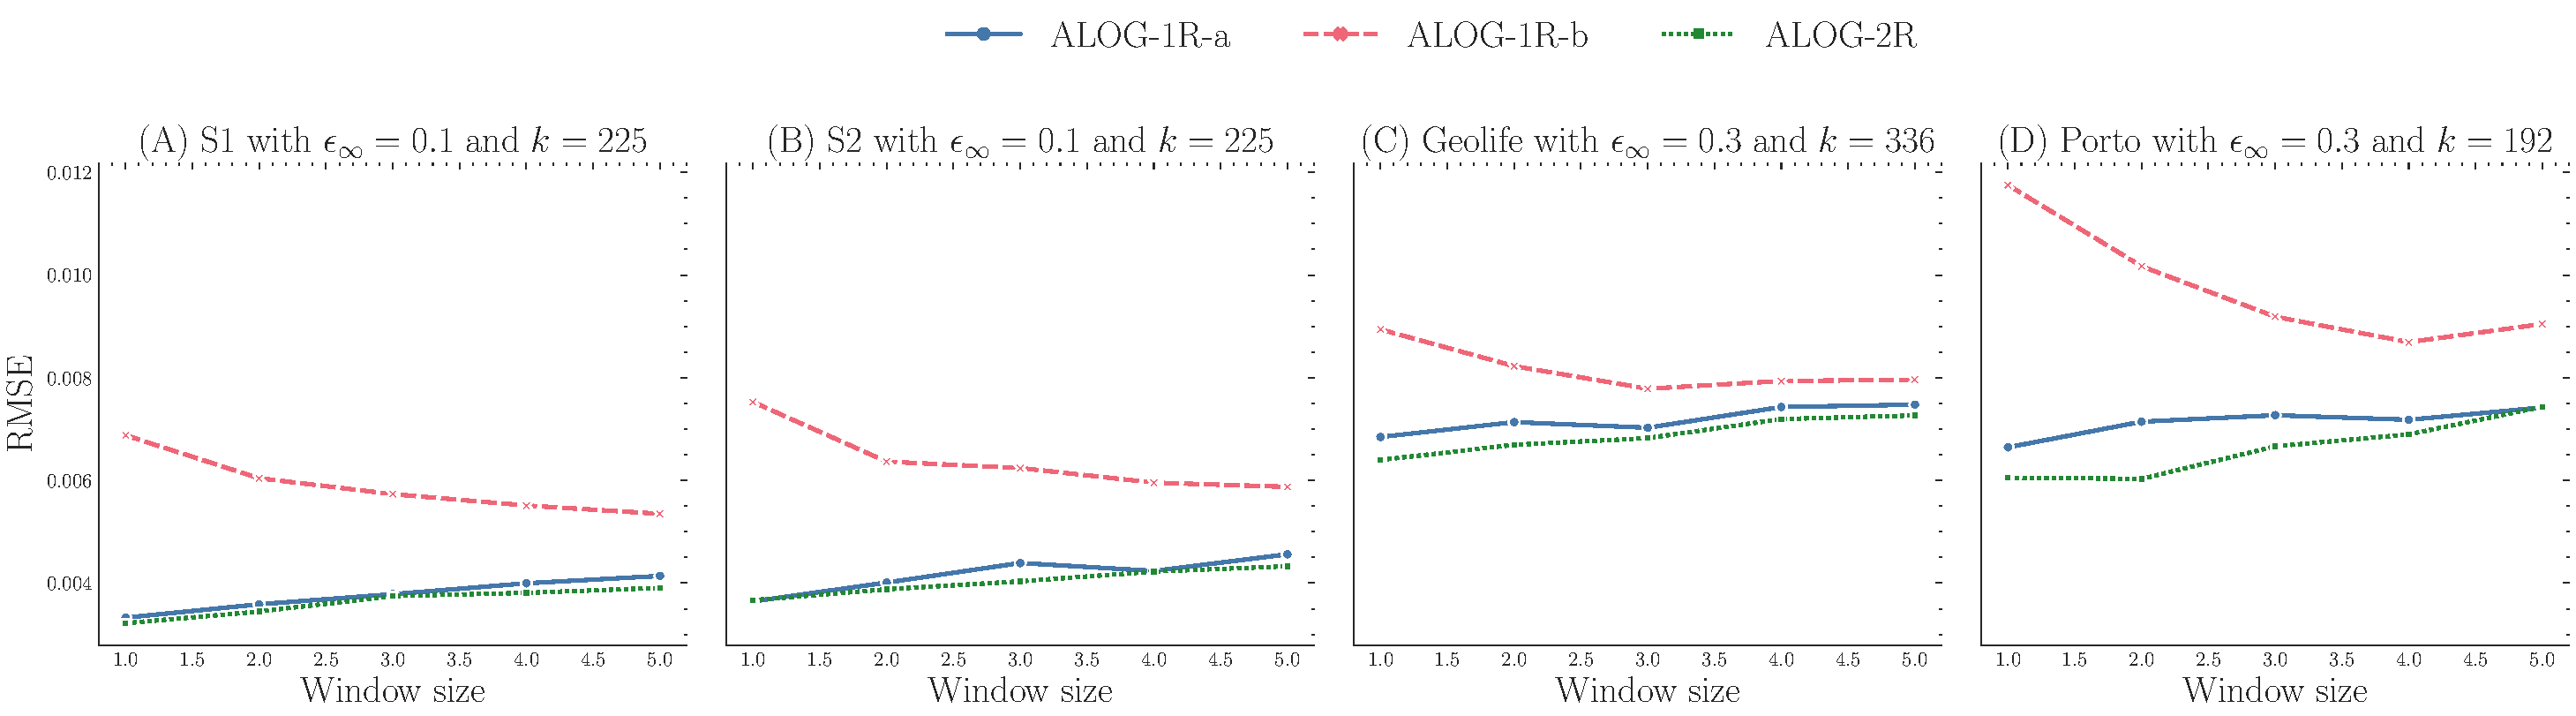
\includegraphics[width=\linewidth]{sections/figures/res_windows.pdf}
%     \caption{RMSE variation in terms of the grid adaptation window size for the four datasets: S1, S2, GeoLife, and Porto.}
%     \label{fig:Window_linechart}
% \end{figure*}


\paragraph{Budget partition x Utility:}The final aspect of our analysis focuses on ALOG-2R, the best-performing method across datasets. A critical factor influencing its performance is the partitioning of the privacy budget between the first and second rounds. This partitioning directly affects the utility achieved by ALOG-2R, as it determines the extent to which each round can contribute to the grid's adaptability and the accuracy of the results.

In the first round, the budget is primarily used to initialize the grid structure and adapt it to the data distribution. This stage is crucial for ensuring that the grid reflects the overall data density and establishes a strong foundation for further refinements. The second round leverages the remaining budget to refine the grid further and address more localized variations in the data.

Table \ref{tab:bpmse} reveals that for datasets S1, S2, and Porto, the optimal partitioning allocates 30\% of the total budget to the first round, with the remaining 70\% allocated to the second round. This configuration ensures sufficient budget for initializing the grid while allowing for meaningful refinements in the second round.

Conversely, the Geolife dataset exhibits only minor differences in RMSE across the tested budget partitioning strategies. The optimal configuration, with 50\% of the budget assigned to each of the two allocation stages, results in a minimal improvement in RMSE. This suggests that the specific characteristics of the Geolife data permit a wider range of effective privacy budget distributions.
% 
\begin{table}[!tb]
\centering
\footnotesize
\caption{RMSE as a function of budget proportion used in ALOG-2R for rounds 1 and 2 (values are in units of $\times 10^{-3}$)}
\begin{tabular}{c|cccccc}
\toprule
\textbf{DataSet} & \textbf{S1} & \textbf{S2} & \textbf{Geolife} & \textbf{Porto} \\
\midrule
$\mathbf{(r_1=0.1\epsilon,r_2=0.9\epsilon)}$ & $3.88$ & $4.18 $ & $7.07 $ & $6.96$\\
$\mathbf{(r_1=0.3\epsilon,r_2=0.7\epsilon)}$ & \cellcolor{black!8}$\mathbf{3.82} $ & \cellcolor{black!8}$\mathbf{4.06} $ & $7.07 $ & \cellcolor{black!8}$\mathbf{6.87}$ \\
$\mathbf{(r_1=0.5\epsilon,r_2=0.5\epsilon)}$ & $3.92 $ & $4.08 $ & \cellcolor{black!8}$\mathbf{7.06} $ & $7.08 $ \\
$\mathbf{(r_1=0.7\epsilon,r_2=0.3\epsilon)}$ & $3.87$ & $4.12 $ & $7.07$ & $7.39$ \\
\bottomrule
\end{tabular}
\label{tab:bpmse}
\end{table}
% 
In summary, the results emphasize the robustness of ALOG-2R in delivering superior utility through its adaptive grid mechanism, making it a strong candidate for practical applications in privacy-preserving data analysis. The findings also underscore the importance of tuning parameters such as grid adaptation windows and budget partitioning to maximize performance across varying scenarios.


\section{Conclusion}
\label{sec:conclusion}

In this work, we proposed ALOG, a framework for privacy preserving frequency estimation using adaptive grids under Local Differential Privacy (LDP). Through extensive evaluations across synthetic and real-world datasets, we demonstrated the superiority of ALOG approaches, particularly ALOG-2R, in balancing utility and privacy compared to traditional methods such as RAPPOR, LOLOHA, and LOSUE. The results highlighted the effectiveness of adaptive grids in dynamically adjusting to varying data densities, significantly reducing MSE while maintaining robust privacy guarantees.

Key findings include the importance of selecting appropriate parameters, such as grid adaptation windows and privacy budget partitioning. ALOG-2R consistently delivered superior performance, with optimal budget partitioning strategies (e.g., 30\%-70\% for most datasets) and smaller grid adaptation windows yielding the best utility. However, a notable limitation of the current ALOG approaches is their inability to reduce grid granularity when data density decreases. This results in granular grids that can lead to increased error over extended periods.

In real-world scenarios, where the distribution of reports evolves throughout the day—such as during peak and off-peak hours in urban settings—it is critical to overcome this limitation to provide a truly adaptive model. Addressing this challenge would enable the grid to dynamically adjust to both increases and decreases in data density, ensuring optimal utility and efficient resource usage.

% \subsubsection*{Future Works:}
% While ALOG has demonstrated significant advantages, nonetheless, further research is needed to explore several promising directions. One of them is the investigation of automated parameter-tuning mechanisms. We believe that applying machine learning techniques to optimize budget partitioning and window size could further optimize utility and efficiency across diverse datasets and application scenarios. Additionally, enhancing the granularity adjustment process is a critical area of improvement. Introducing mechanisms to dynamically increase and decrease grid granularity, such as merging or splitting cells based on data density, could address the current limitations of ALOG-2R and ALOG-1R-a, enabling more precise adaptations over time.

% These advancements would further refine the balance between privacy, utility, and adaptability, paving the way for even more robust and flexible solutions in privacy-preserving geospatial data analysis.

\subsubsection*{Future Works:}
While ALOG shows strong performance, further work is needed to explore several key directions. One is automating parameter tuning—using machine learning to optimize budget partitioning and window size could enhance utility and efficiency across varying datasets.
Enhancing granularity adjustment through dynamic cell merging and splitting will directly overcome ALOG-2R and ALOG-1R-a's current limitations, enabling more adaptive data representation.
These directions could further improve the balance among privacy, utility, and adaptability in privacy-preserving geospatial analysis.

\subsection*{Acknowledgements}
This research was partially supported by the Coordenação de Aperfeiçoamento de Pessoal de Nível Superior CAPES (grant \# 88882.454568/2019-01) and the Conselho Nacional de Desenvolvimento Científico e Tecnológico CNPq
(grant \# 316729/2021-3).
It was partially funded by Lenovo, as part of its R\&D investment under Brazilian Informatics Law. 


\section{Artifacts}

The artifacts for reproducing our experiments are available at:

\begin{center}
    \url{https://github.com/edurdneto/ALOG}
\end{center}

The repository includes source code, method implementations, experiment scripts, and reproduction instructions.



%%
%% The next two lines define the bibliography style to be used, and
%% the bibliography file.
\bibliographystyle{ACM-Reference-Format}
\bibliography{edubibtex}


%%
%% If your work has an appendix, this is the place to put it.
%%\appendix


\end{document}
\endinput
%%
%% End of file `edbt-paper-template-29-1.tex'.
